\documentclass[a4paper,12pt]{article}

% Import the deliverable package from common directory
\usepackage{../common/deliverable}

\usepackage{beamerarticle}
%%\documentclass[ignorenonframetext,red]{beamer}

%\mode<article>{\usepackage{fullpage}}
\mode<presentation>{\usetheme{RomaTorVergata}}
% Tell LaTeX where to find graphics files
\graphicspath{{../common/logos/}{./figures/}{../}}

\usepackage{xspace}
\usepackage{listings}

% Set the deliverable number (without the D prefix, it's added automatically)
\setdeliverableNumber{1.6}
% Various utilities for the slides.

%\usepackage[utf8x]{inputenc}
%\usepackage[T1]{fontenc}

\usepackage{listings}
\lstset{
    language=C++,
    basicstyle=\ttfamily\scriptsize,
    keywordstyle=\color{blue},
    commentstyle=\color{gray},
    stringstyle=\color{red},
    breaklines=true,
    frame=single,
    numbers=left,
    numberstyle=\tiny,
    showstringspaces=false
}

% \lstset{basicstyle=\ttfamily,
% 	showstringspaces=false,
% 	commentstyle=\color{red},
% 	keywordstyle=\color{blue},
% 	emph={%  
% 		psb_init, psb_info, psb_exit,%
% 		psb_get_mpi_comm,psb_get_mpi_rank,%
% 		psb_snd,psb_rcv,%
% 		psb_bcast,
% 		psb_sum,
% 		psb_amx,
% 		psb_amn,
% 		psb_max,
% 		psb_min,
%                 psb_scan_sum,
%                 psb_exscan_sum,
% 		psb_geaxpby,
% 		psb_spmm,
% 		psb_gedot,
% 		psb_genrm2,
% 		psb_halo,
% 		psb_cdall,
% 		psb_sum,
% 		psb_cdins,
% 		psb_cdasb,
% 		psb_spall,
% 		psb_spins,
% 		psb_spasb,
% 		psb_sprn,
% 		psb_sp_clone,
% 		psb_geall,
% 		psb_geins,
% 		psb_geasb,
% 		psb_glob_to_loc,
% 		psb_loc_to_glob,
% 		psb_krylov,
% 		psb_precinit,
% 		psb_precbld,
% 		psb_geamax,
% 		psb_geasum,
% 		psb_spnrmi,
% 		psb_spsm,
% 		mm_array_write,
% 		mm_mat_write,
% 		mm_array_read,
% 		mm_mat_read,
% 		hb_read,
% 		hb_write,
% 		init,
% 		set,
% 		hierarchy_build,
% 		smoothers_build,
% 		build,
% 		cscnv,
% 		apply,
% 		free,
% 		descr,
%                 mode,
%                 request
% 	},emphstyle={\color[HTML]{E4605B}}%
% }

\definecolor{keycolor}{RGB}{172, 42, 42}
\definecolor{mbleu}{RGB}{64,96,127}
\definecolor{vimvert}{RGB}{46, 139, 87}
\definecolor{Red}{rgb}{1.0, 0.01, 0.24}
\definecolor{Lime}{rgb}{0.75, 1.0, 0.0}
\definecolor{Yellow}{rgb}{1.0, 0.77, 0.05}
\definecolor{gray}{rgb}{0.66, 0.66, 0.66}
\definecolor{ao(english)}{rgb}{0.0, 0.5, 0.0}
\definecolor{codecolor}{HTML}{eae1de}
\definecolor{ttqqqq}{rgb}{0.2,0,0}

\def\zz{\color{mbleu}\textless\bgroup\itshape\aftergroup\endzz}
\def\endzz{\textgreater\egroup}

\lstdefinestyle{global}{
	basicstyle=\ttfamily\scriptsize\color{black!90},%
	stringstyle=\itshape\color{magenta},%
	showstringspaces=false,%
	keywordstyle=\bfseries\color{keycolor},%
	commentstyle=\color{blue}\slshape,%
	framexleftmargin=1mm,%
}

\lstdefinestyle{makefile}{
	otherkeywords={.SUFFIXES},
	morekeywords={SUFFIX, CPP_,},
	moredelim=[is][\color{mbleu}]{/*}{*/},
	style=global,%
	morecomment=[l][commentstyle]{\#},%
	emphstyle={\color{vimvert}},%
	moredelim=[s][\color{vimvert}]{\$(}{)}%
}
\def\bx{{\mathbf x}}
\def\bb{{\mathbf b}}
\def\br{{\mathbf r}}
\def\be{{\mathbf e}}
\def\bK{{\mathbf K}}
\def\bu{{\mathbf u}}
\def\bw{{\mathbf w}}
\newcommand{\R}{{\mathcal R}}
\newcommand{\Range}{{\mathcal Range}}
\usepackage{bbding}
\usepackage{fontawesome5}

\usepackage{multicol}
\usepackage{pgfplots}
\usepackage{pgfkeys}
\usepackage{tikz}
\usetikzlibrary{chains,shapes.arrows,shapes.multipart,
  arrows,arrows.meta,positioning,decorations,,
  decorations.pathreplacing,matrix,
  decorations.pathmorphing,plothandlers}
\tikzset{
    >=stealth',
    punktchain/.style={
        rectangle, 
        rounded corners, 
        % fill=black!10,
        draw=white, very thick,
        text width=6em,
        minimum height=2em, 
        text centered, 
        on chain
      }
    }
\usepackage{pgf-pie}
\usepackage{amsmath,amssymb,amsfonts}
\usepackage{smartdiagram}
\usepackage{natbib}
\usepackage[tworuled,linesnumbered]{algorithm2e}
\usepackage{colortbl}%
\newcommand{\myrowcolour}{\rowcolor[gray]{0.925}}
\usepackage{booktabs}
\usepackage{subcaption}

%\usepackage{pgfpages}
\usepackage{pgfmorepages}
\pgfmorepagesloadextralayouts


\newcommand*{\tred}[1]{\textcolor{red}{#1}}
\newcommand*{\tgreen}[1]{\textcolor{green}{#1}}
\newcommand*{\tblu}[1]{\textcolor{blue}{#1}}
% Begin document
\begin{document}
\pgfpagesuselayout{1 on 1}[a4paper]
% Create the title page with the title as argument
\maketitlepage{Tutorials based on external libraries}

\newpage

% Main Table using the new environment and command
\begin{deliverableTable}
  \tableEntry{Deliverable title}{Tutorials based on external libraries}
  \tableEntry{Deliverable number}{D1.6}
  \tableEntry{Deliverable version}{0.1}
  \tableEntry{Date of delivery}{Feb 28th 2026}
  \tableEntry{Actual date of delivery}{[Actual date]}
  \tableEntry{Nature of deliverable}{DEM - Demonstrator, pilot, prototype}
  \tableEntry{Dissemination level}{Public}
  \tableEntry{Work Package}{WP1}
  \tableEntry{Partner responsible}{UNITOV}
\end{deliverableTable}

% Abstract and Keywords Section
\begin{deliverableTable}
  \tableEntry{Abstract}{This report contains the tutorial on the
    external library PSCToolkit, delivered to the dealii-X project
    during the winter school event at SISSA on Dec. 11th and 12th, 2025.}
  \tableEntry{Keywords}{Linear algebra solvers. Libraries. Data
    structures.}
\end{deliverableTable}

\newpage

\begin{documentControl}
  \addVersion{0.1}{Feb 15th 2026}{Salvatore Filippone}{Initial draft}
  \addVersion{0.2}{Feb 27th 2026}{Marco Feder}{Tutorial program}
\end{documentControl}

\subsection*{{Approval Details}}
Approved by: [Name] \\
Approval Date: [Date]

\subsection*{{Distribution List}}
\begin{itemize}
  \item [] - Project Coordinators (PCs)
  \item [] - Work Package Leaders (WPLs)
  \item [] - Steering Committee (SC)
  \item [] - European Commission (EC)
\end{itemize}

\vspace*{2cm}

\disclaimer

\newpage

\tableofcontents % Automatically generated and hyperlinked Table of Contents

\newpage

\section{{Introduction}}

Work Package 1 is dedicated to the numerical software backbone of
dealii-X, enabling the transition to exascale computing. One key
aspect of the WP is the interfacing with external libraries,
especially PSCToolkit~\url{https://psctoolkit.github.io} and MUMPS.
This interface is mostly transparent to the application end-user;
however, the developers need to acquire a working knowledge of the
features available and of the performance that can be attained. The integration
status of PSCToolkit and MUMPS in dealii-X has been documented in D1.7, which we refer to
for details.

\subsection{{Purpose of the Document}}
The purpose of this document is to make available in deliverable
format the tutorial presentations given at the dealii-X winter school event at
SISSA on Dec. 10th and 11th, 2025. The present tutorial program can be found
at \url{https://github.com/psctoolkit/dealii/blob/configure_amg4psblas/examples/benchmark}. We also report in the Appendix the slides of the presentation given at the winter school event.

\section{PSCToolkit: PSBLAS 3.9 \& AMG4PSBLAS 1.2 Tutorial}


The new interface targets latest release candidates PSBLAS 3.9 and AMG4PSBLAS 1.2. In order
to demonstrate the correctness of the new interface, we describe here a tutorial program which shows
how to use the wrappers in a simple but illustrative test case, in the spirit of classical
tutorials programs of the deal.II library\footnote{\url{https://dealii.org/developer/doxygen/deal.II/Tutorial.html}}.

We consider the following variable-coefficient Poisson problem on a bounded polygonal domain $\Omega \subset \mathbb{R}^d$, $d=2,3$:
$$-\nabla \cdot ( \mathbf{K} \nabla u) = f \quad \text{ in } \Omega = [0,1]^d, \quad d=2,3,$$
where $\mathbf{K}$ is a symmetric and uniformly positive definite tensor and $u$ satisfies homogeneous Dirichlet boundary conditions on $\partial \Omega$. We discretize the continuous problem with standard nodal Lagrangian $\mathcal{Q}^1$ elements on quadrilateral meshes.

All the preliminary steps involved in a standard finite element pipeline, i.e. mesh generation, partitioning
of the computational grid among MPI processes, construction of finite element spaces and distribution of
degrees of freedom are orthogonal to the present interface, which only needs to interact
with deal.II exclusively at the linear algebra level, taking as input the
assembled distributed sparse matrix and right-hand side vector.

For this reason, we do not report here the details regarding the setup of the problem, which can be found in the tutorial program \texttt{step-40} of the
deal.II library, and we focus instead only on the minor modifications required to use the PSCToolkit wrappers. Since our problem
yields a symmetric positive definite linear system, we use the conjugate gradient method preconditioned by one V-cycle of the algebraic
multigrid preconditioner implemented by AMG4PSBLAS. Details about the setup of the preconditioner will be presented later.

\subsection{Include files and problem setup}
In addition to classical deal.II include files, the tutorial program includes
the headers which contains the interface common to all linear algebra
backends used in the deal.II library.

\begin{lstlisting}[language=C++,caption=New header files]
#include <deal.II/lac/psblas_precondition.h>
#include <deal.II/lac/psblas_sparse_matrix.h>
#include <deal.II/lac/psblas_vector.h>
\end{lstlisting}

In addition, the tutorial program supports parameter files that can be used at runtime
to configure the details of the problem and the solver without recompiling. These
parameter files allow the user to control, among other settings:
\begin{itemize}\itemsep0pt\parskip0pt
  \item the number of refinement cycles and whether adaptive mesh refinement (AMR) is enabled,
  \item the solver tolerances (relative and absolute) for the iterative linear solver,
  \item the details of the AMG preconditioner, such as coarsening strategy, smoother type,
        and number of smoothing steps.
\end{itemize}

As common in tutorial programs, the triangulation, system matrix, right-hand side vector, and solution vector are
declared as class members of the main class, and the setup of the linear system is performed in a dedicated
member function. The main difference with respect to a standard tutorial program
is that the system matrix and vectors are declared using the PSBLAS wrappers. Listing \ref{lst:class_declaration} shows the code snippet for the class declaration of the main class of the tutorial program, where only the PSCToolkit-specific members are shown.

\begin{lstlisting}[language=C++, caption={Class declaration (only PSCToolkit-specific members shown).}, label=lst:class_declaration]
template <int dim>
class LaplaceProblem
{
public:
  // declaration of constructors and run()

private:
  // data structures for triangulation, degrees of freedom, etc. as in step-40

  PSCToolkit::SparseMatrix<double> system_matrix;
  PSCToolkit::Vector<double>       locally_relevant_solution;
  PSCToolkit::Vector<double>       system_rhs;
};
\end{lstlisting}


The allocation of matrices and vectors are performed in the \texttt{setup\_system()} member function, which
is called at the end of each refinement cycle. The user interface is identical to the one of the other linear
algebra classes: we first need to acquire information about the MPI communicator and the degrees of freedom owned\footnote{Plus some so-called "ghost" or "halo" indices, i.e. indices owned by neighboring processes.} by
the current process. Then, the \texttt{reinit()} member function performs the
allocation of distributed sparse matrices and vectors. Listing \ref{lst:setup_system} shows the code snippet for the setup of the linear system and vectors.

\begin{lstlisting}[language=C++, caption={Setup of the linear system and vectors.}, label=lst:setup_system]
template <int dim>
void LaplaceProblem<dim>::setup_system()
{

  locally_owned_dofs   = dof_handler.locally_owned_dofs();
  locally_relevant_dofs =
    DoFTools::extract_locally_relevant_dofs(dof_handler);

  locally_relevant_solution.reinit(locally_owned_dofs,
                                   locally_relevant_dofs,
                                   mpi_communicator);
  system_rhs.reinit(locally_owned_dofs, mpi_communicator);

  PSCToolkit::SparsityPattern sparsity_pattern(locally_owned_dofs,
                                               mpi_communicator);
  system_matrix.reinit(sparsity_pattern, mpi_communicator);
  system_matrix.reinit(locally_owned_dofs, locally_owned_dofs, dsp,
                       mpi_communicator);
}
\end{lstlisting}


The assembly loop is performed as in any standard tutorial program, looping over cells owned by the current process and scattering local contributions to the global system matrix and right-hand side vector. The implementation of the assembly loop
can be found in the \texttt{assemble\_system()} member function, which is to all extends identical to many other tutorial programs.



\subsection{Solver and preconditioner setup}

We finally describe the \texttt{solve()} function, which involves the setup of the linear solver and the preconditioner, as well as the
solution of the linear system. As previously mentioned, the positive definiteness of the bilinear form
calls for the use of the preconditioned conjugate gradient (PCG) method. At the solver stage, the interface to PSCToolkit becomes essentially
transparent to the user: any Krylov subspace solver provided by the native deal.II library can be instantiated
with PSCToolkit matrix and vector wrappers, since they comply with the linear-algebra interface expected by deal.II. Hence, we use the native
\texttt{SolverCG} class, which implements the PCG method, and is templated on the vector type, which is in this case \texttt{PSCToolkit::Vector<double>}. The workflow is shown in following Listing \ref{lst:linear_solve} where, for the sake of clarity, we omit the preconditioner settings, which can be found in Listing \ref{lst:preconditioner_setup}.

Among the several available configuration options, we highlight the integration with the MUMPS package (cfr. deliverable D1.7), which can be employed as a direct coarse-level solver within the AMG preconditioner. This combination is particularly effective for achieving robust convergence when algebraic multigrid methods benefit from an accurate solution at the coarsest level. Moreover, efficient parallel-efficient coarse solvers can improve the overall scalability of the solver, especially in contexts where the size of coarse-level system is large.


The solver part therefore remains hence unchanged with respect to standard user codes, and only the AMG4PSBLAS preconditioner settings (coarsening strategy, coarse solver, smoothers, tolerances) may need tuning.


\begin{lstlisting}[language=C++,caption={Native SolverCG class with PSCToolkit data structures.}, label=lst:linear_solve]
template <int dim>
void LaplaceProblem<dim>::solve()
{

  PSCToolkit::Vector<double> completely_distributed_solution(
    locally_owned_dofs, mpi_communicator);
  SolverCG<PSCToolkit::Vector<double>> solver(solver_parameters);

  typename PSCToolkit::PreconditionAMG::AdditionalData prec_data;
  // fill prec_data with the desired settings for the AMG preconditioner
  PSCToolkit::PreconditionAMG preconditioner;
  preconditioner.initialize(system_matrix, prec_data);
  solver.solve(system_matrix,
              completely_distributed_solution,
              system_rhs,
              preconditioner);
    }
\end{lstlisting}




\begin{lstlisting}[caption={Excerpt of parameter file with AMG preconditioner settings.},label=lst:preconditioner_setup]
subsection Laplace Problem<2>
  // problem-related parameters (refinement cycles, boundary ids, etc.)

  subsection AMG control
    set Aggregation filter             = FILTER
    set Aggregation threshold          = 1e-2
    set Aggregation type               = SOC1
    set Aggregation size               = 8
    set Coarse matrix type             = DIST
    set Coarse solver                  = MUMPS
    set Cycle type                     = VCYCLE
    set Number of cycles               = 1
    set Parallel aggregation algorithm = DECOUPLED
    set Prolongator aggregation        = SMOOTHED
    set Smoother sweeps                = 3
    set Smoother type                  = FBGS
    set Verbose AMG info               = true
  end
end
\end{lstlisting}




\subsection{Numerical experiment}

We consider the $\mathcal{Q}^1$ discretization of the anisotropic Poisson problem with diffusion tensor
\begin{equation}
  \mathbf{K}
  =
  \begin{pmatrix}
    \cos^2\theta + \varepsilon \sin^2\theta
     &
    (1-\varepsilon)\sin\theta\cos\theta
    \\
    (1-\varepsilon)\sin\theta\cos\theta
     &
    \sin^2\theta + \varepsilon \cos^2\theta
  \end{pmatrix},
\end{equation} and right-hand side $f=1$. The CG solver is stopped when the relative residual is reduced by a factor of $10^{-6}$, or when the absolute residual is smaller than $10^{-10}$.

Figure \ref{fig:AMR} shows the solution obtained with several AMR cycles starting from a Cartesian grid, and letting the AMR be driven by a suitable error estimator. The anisotropy parameters are $\varepsilon = 100$ and $\theta = \frac{\pi}{6}$, which yield a challenging test case for algebraic multigrid methods, especially when AMR is employed.



\begin{figure}[htbp]
  \centering
  \begin{subfigure}{0.20\columnwidth}
    
\includegraphics[width=\columnwidth]{sol0.eps}
    \caption{$\ell = 0$}
  \end{subfigure}\hfil
  \begin{subfigure}{0.20\columnwidth}
    
\includegraphics[width=\columnwidth]{sol1.eps}
    \caption{$\ell = 1$}
  \end{subfigure}\hfil
  \begin{subfigure}{0.20\columnwidth}
    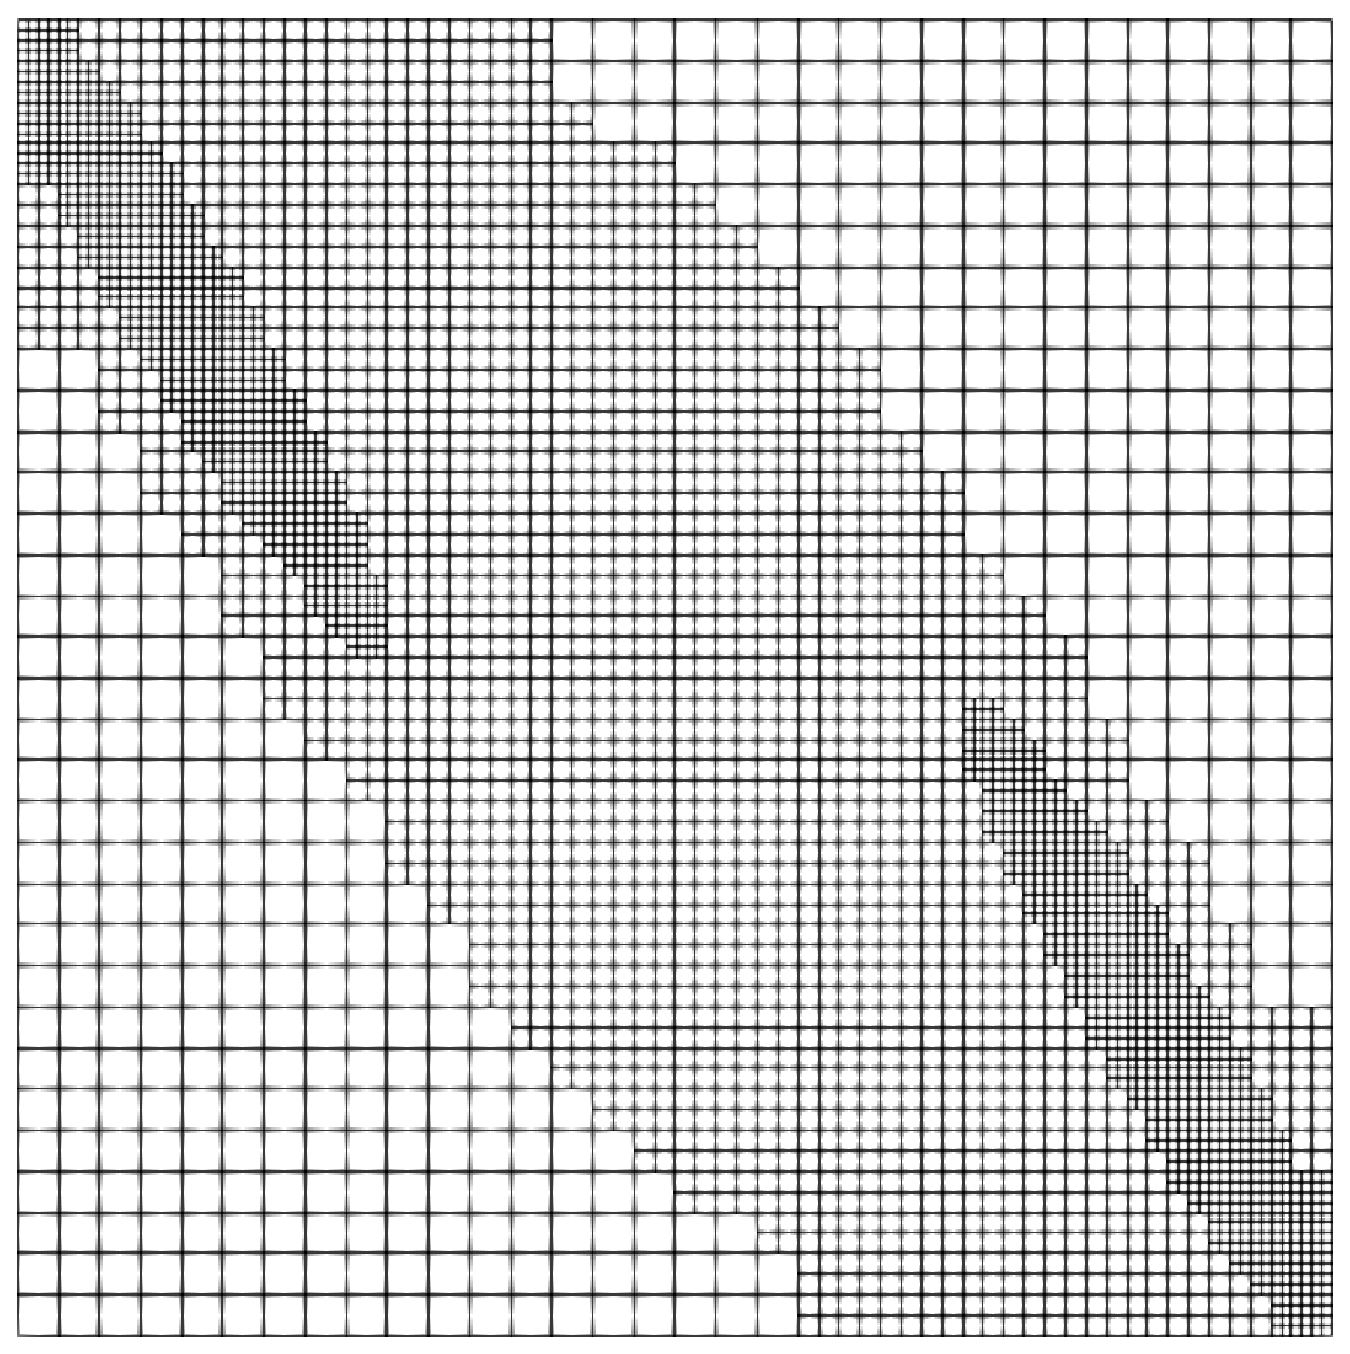
\includegraphics[width=\columnwidth]{sol2.eps}
    \caption{$\ell = 2$}
  \end{subfigure}\hfil
  \begin{subfigure}{0.20\columnwidth}
    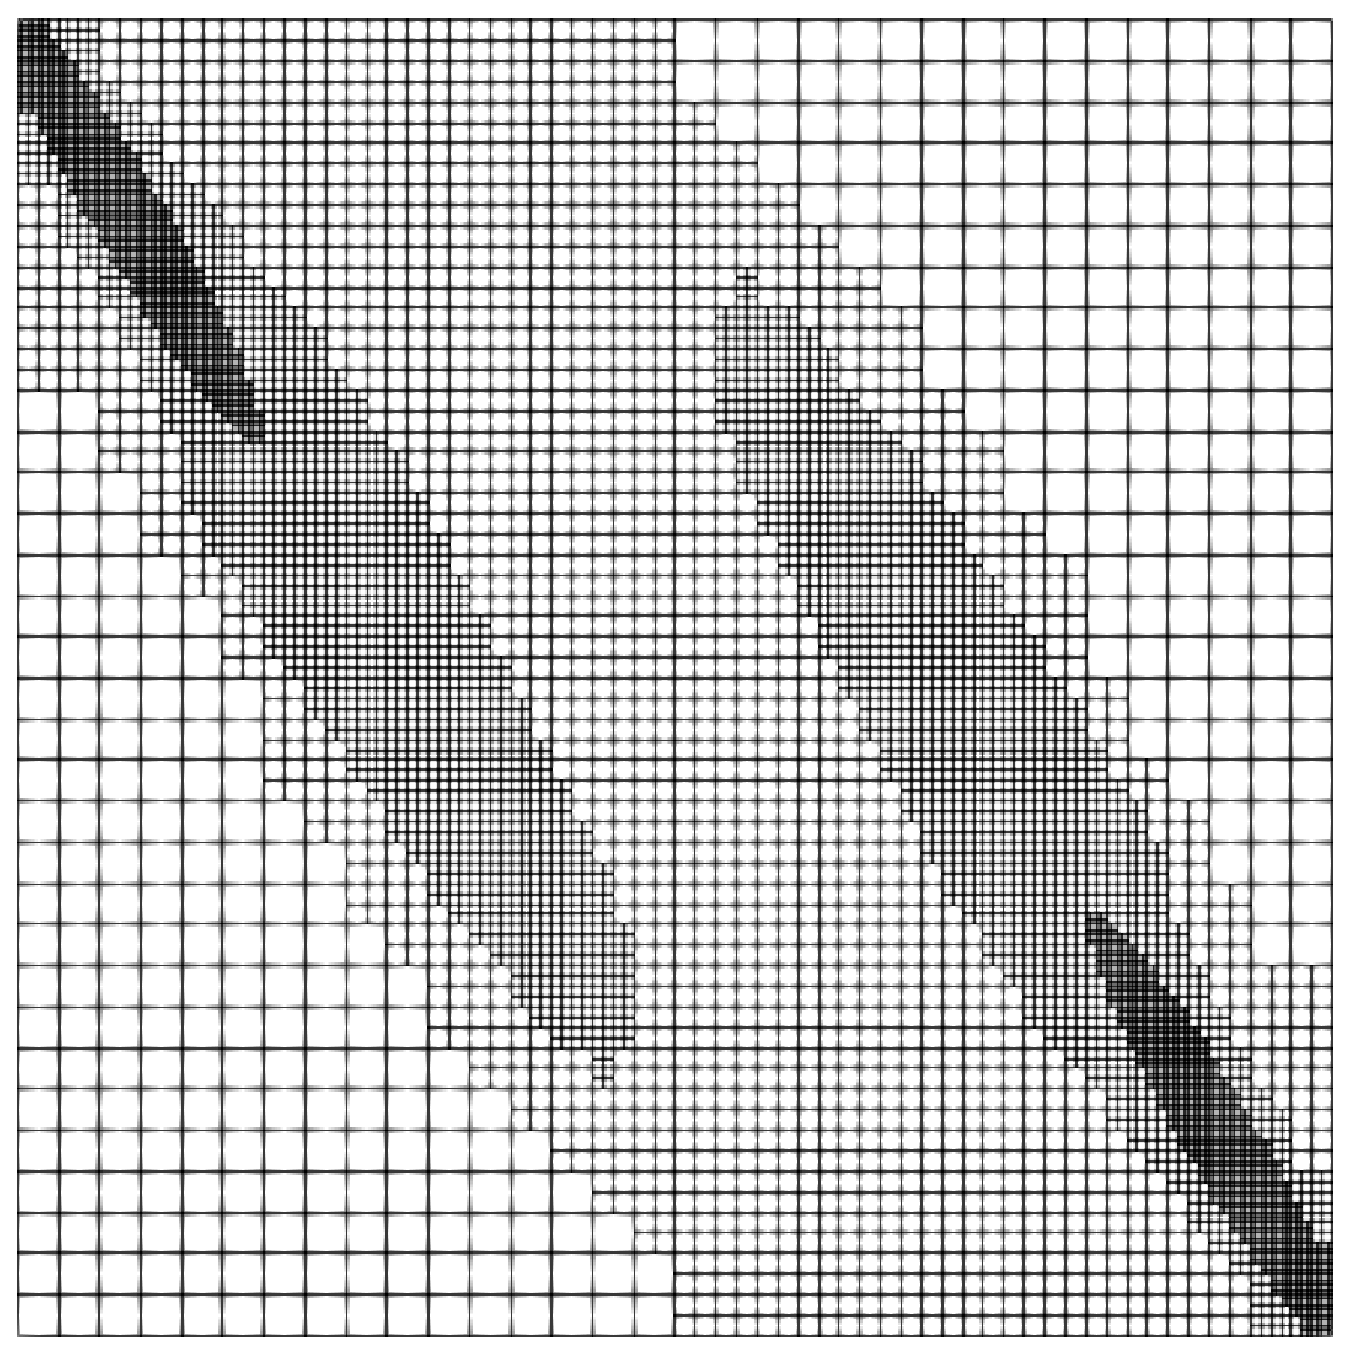
\includegraphics[width=\columnwidth]{sol3.eps}
    \caption{$\ell = 3$}
  \end{subfigure}

  \begin{subfigure}{0.20\columnwidth}
    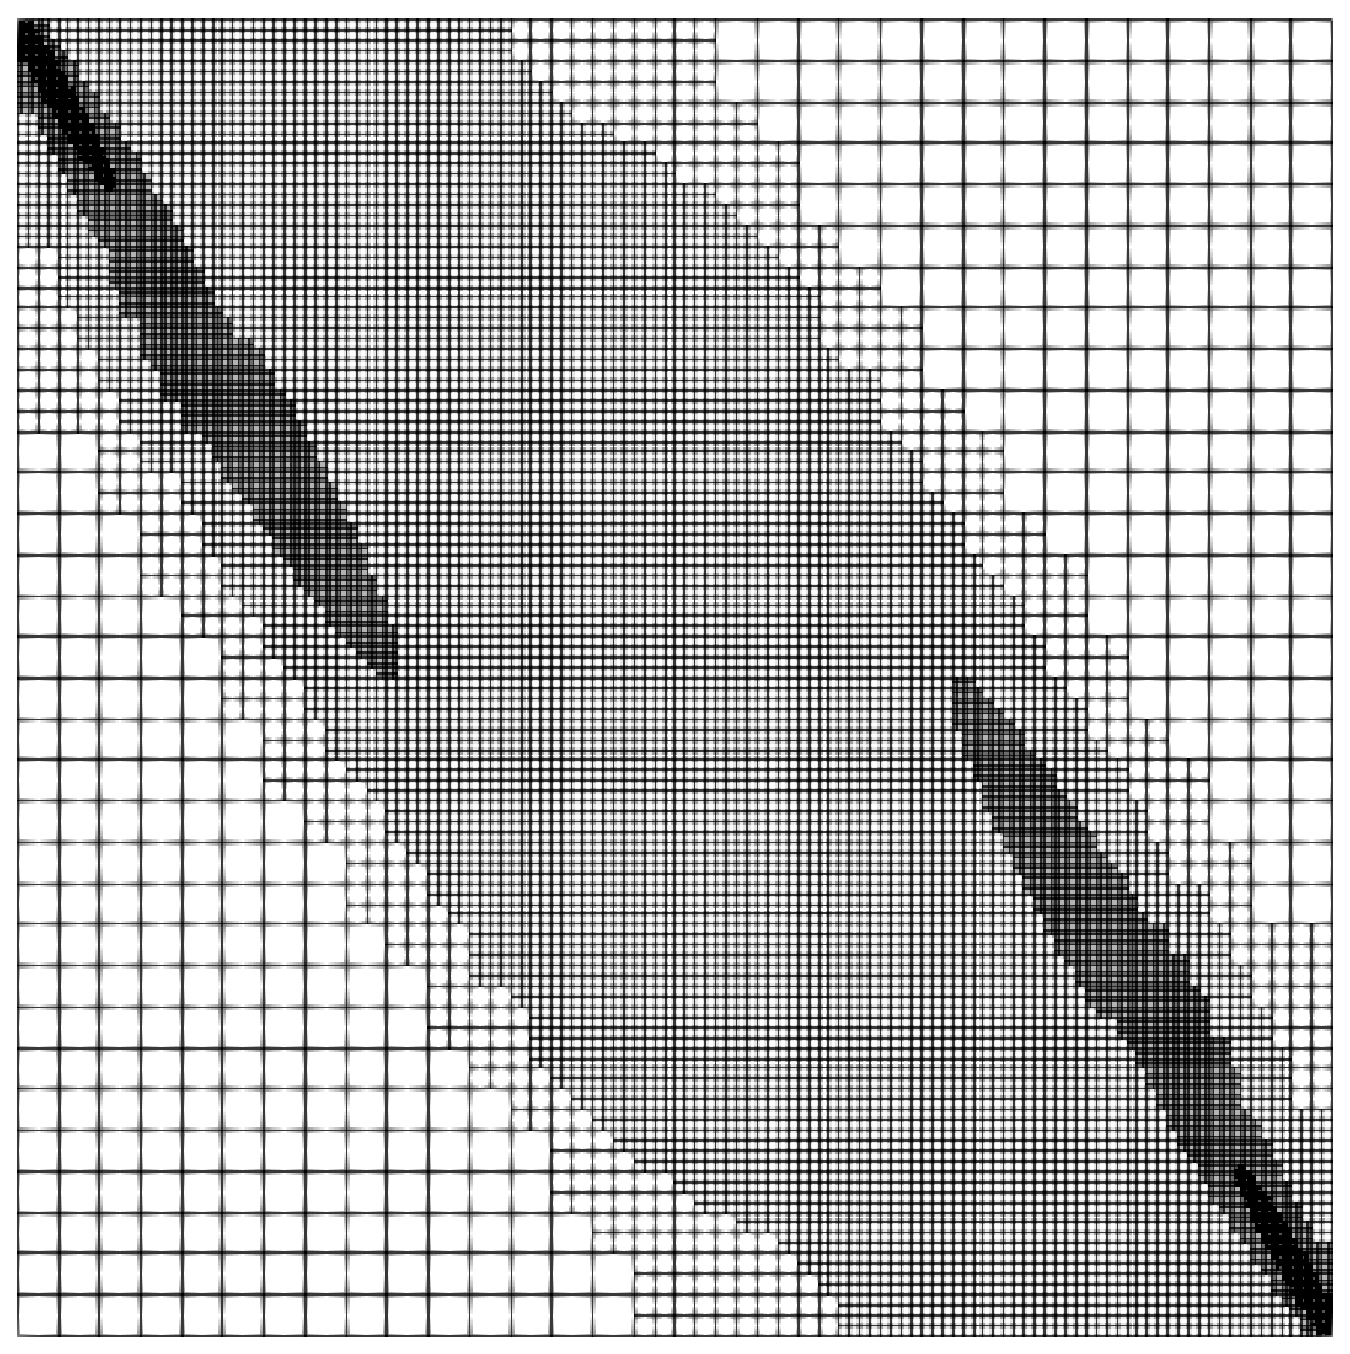
\includegraphics[width=\columnwidth]{sol4.eps}
    \caption{$\ell = 4$}
  \end{subfigure}\hfil
  \begin{subfigure}{0.20\columnwidth}
    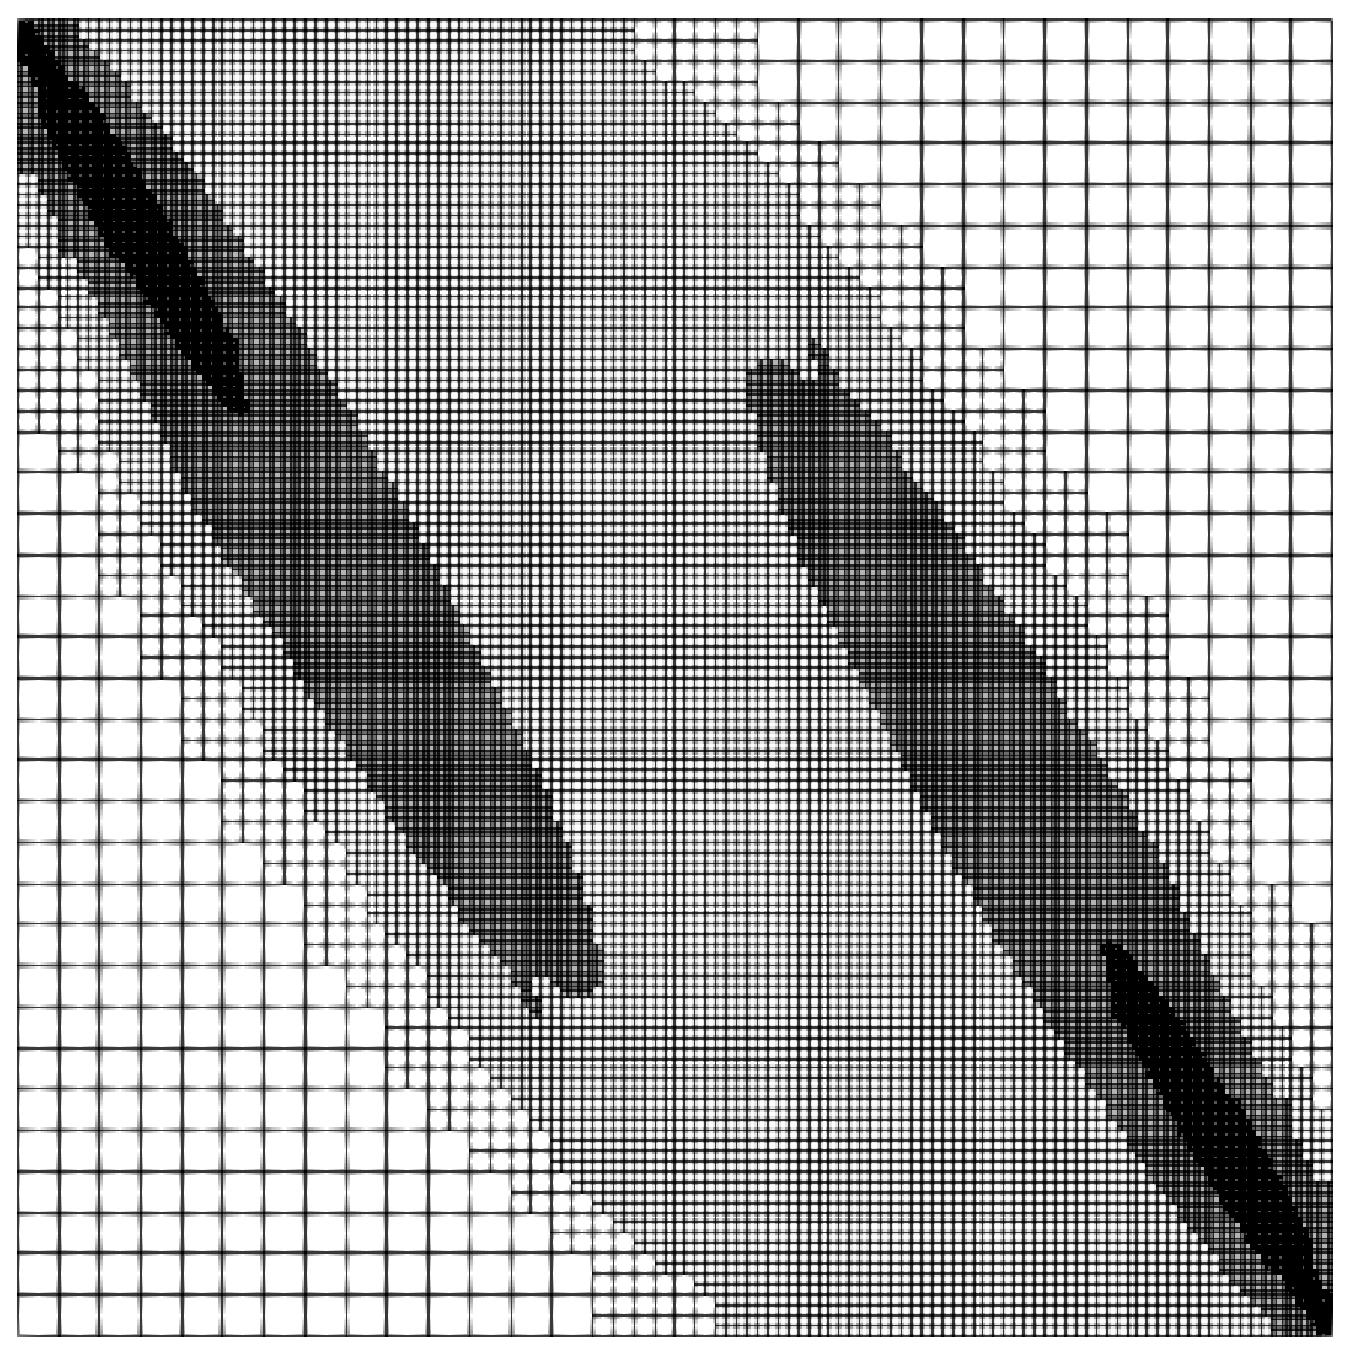
\includegraphics[width=\columnwidth]{sol5.eps}
    \caption{$\ell = 5$}
  \end{subfigure}\hfil
  \begin{subfigure}{0.20\columnwidth}
    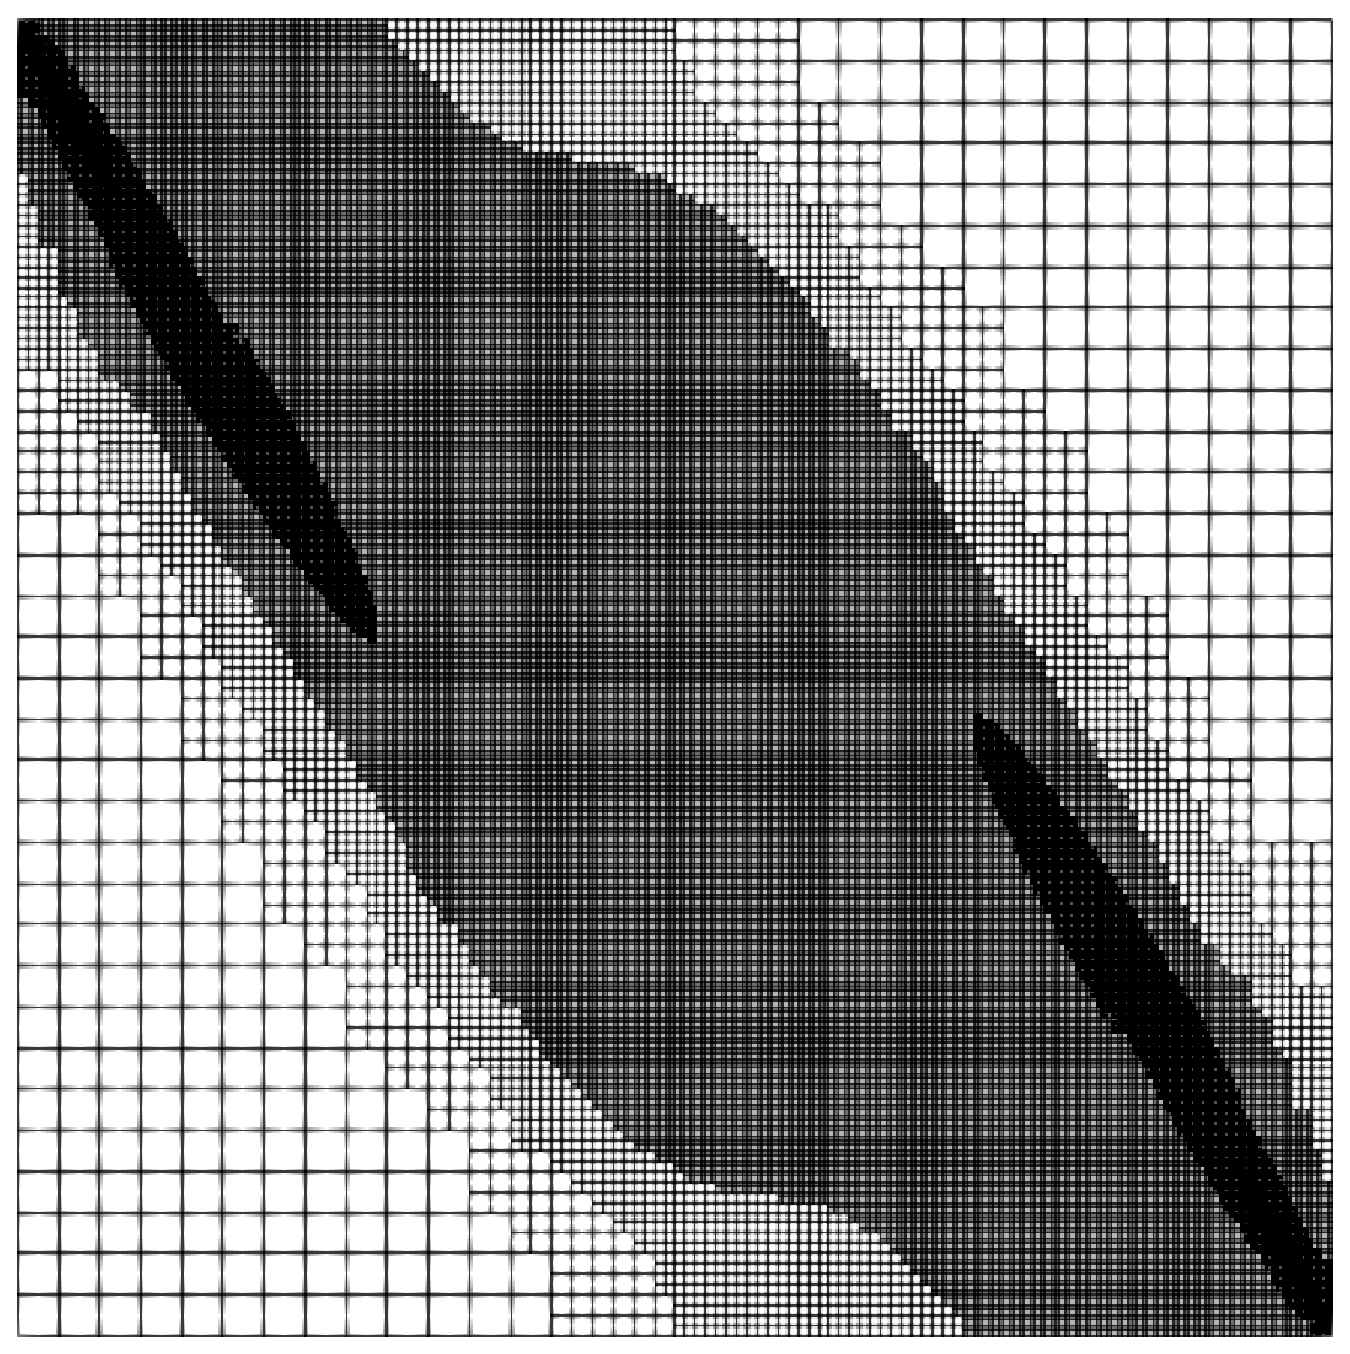
\includegraphics[width=\columnwidth]{sol6.eps}
    \caption{$\ell = 6$}
  \end{subfigure}\hfil
  \begin{subfigure}{0.20\columnwidth}
    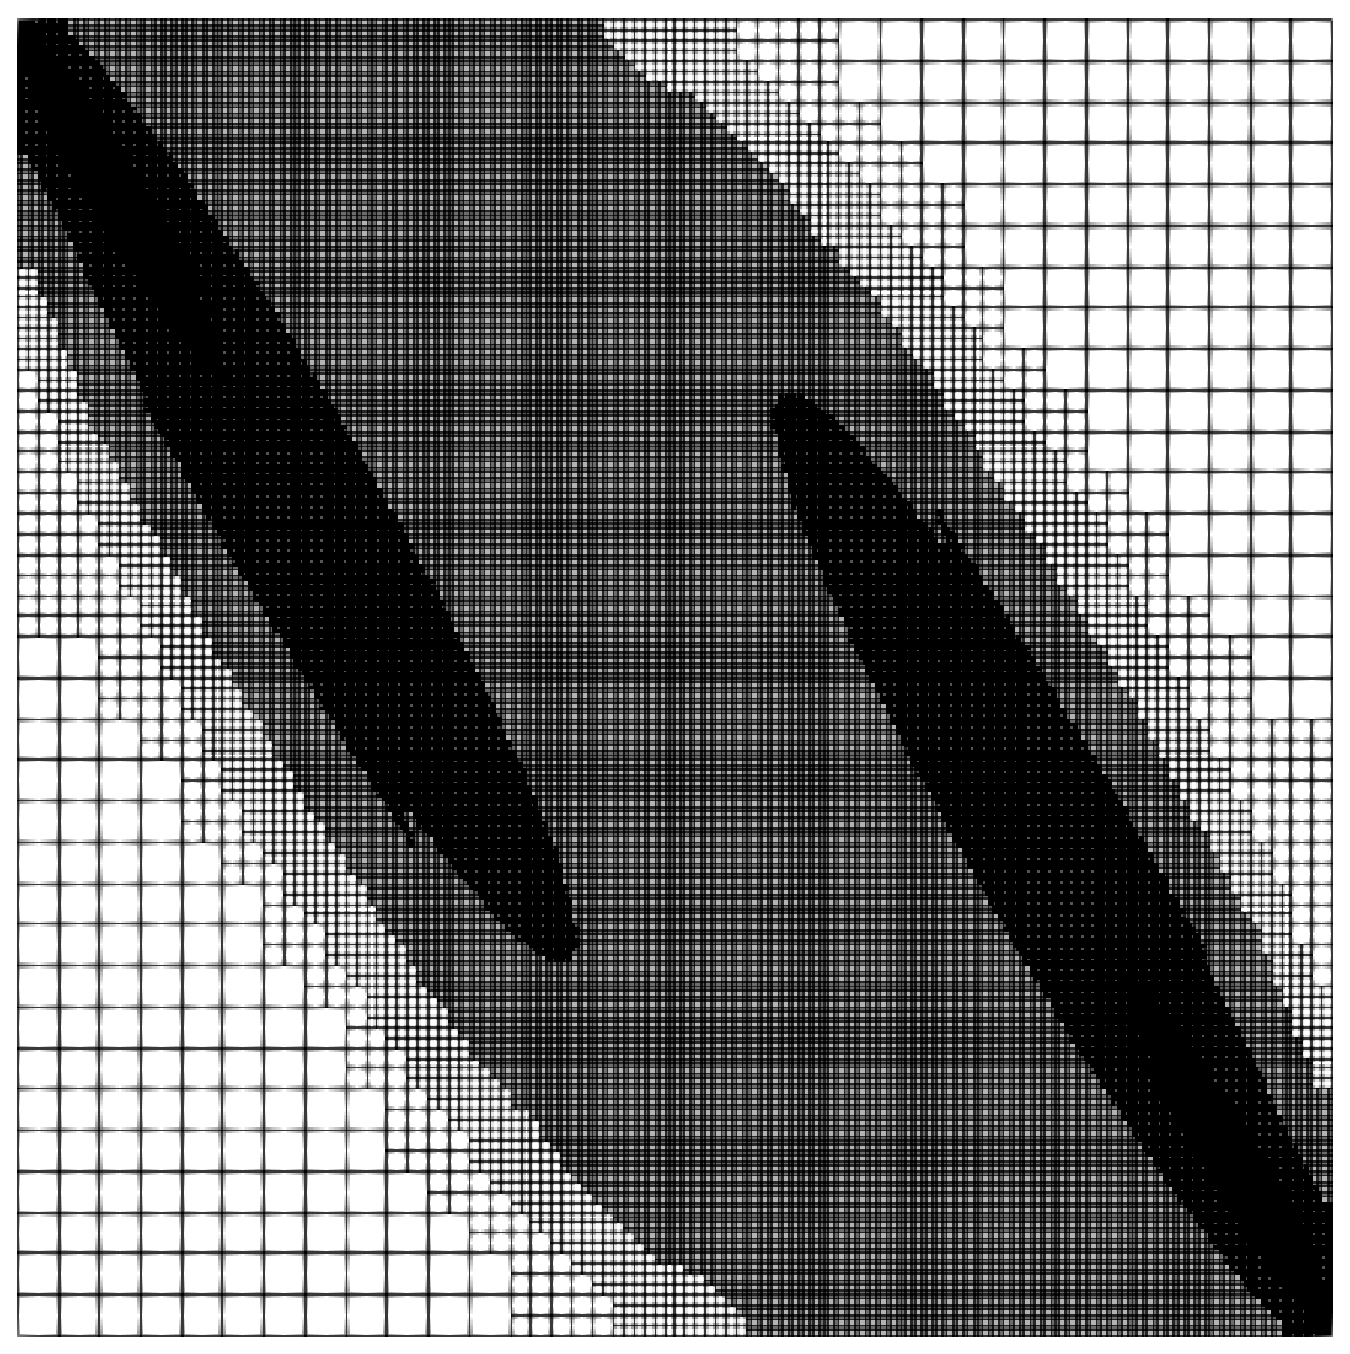
\includegraphics[width=\columnwidth]{sol7.eps}
    \caption{$\ell = 7$}
  \end{subfigure}
  \caption{Example of AMR on a quadrilateral grid for an anisotropic Poisson problem with $\ell = 1,\ldots,7$ levels of refinements from an original tensor product grid $\ell =0$.\label{fig:AMR}}
\end{figure}


Iteration counts obtained with the setup presented in Listing~\ref{lst:preconditioner_setup} are reported in Table~\ref{tab:anisopoisson2D}, where we show the results for the two-dimensional case with several AMR cycles, and for different numbers of MPI processes. Iterations are fairly robust with respect to the number of MPI processes and the AMR level.

\begin{table}[htbp]
  \centering
  \footnotesize
  \begin{tabular}{ccccccccc}
    \toprule
          & \multicolumn{8}{c}{AMR level}                                    \\
    \cmidrule{2-9}
    $n_p$ & 0                             & 1  & 2  & 3  & 4  & 5  & 6  & 7  \\
    \midrule
    1     & 17                            & 20 & 24 & 26 & 31 & 32 & 38 & 39 \\
    2     & 14                            & 19 & 24 & 26 & 30 & 32 & 38 & 40 \\
    4     & 8                             & 14 & 21 & 25 & 30 & 31 & 37 & 39 \\
    8     & 9                             & 10 & 16 & 23 & 29 & 33 & 39 & 39 \\
    16    & 9                             & 10 & 10 & 16 & 23 & 26 & 36 & 39 \\
    32    & 9                             & 10 & 10 & 11 & 17 & 25 & 27 & 36 \\
    64    & 10                            & 10 & 10 & 11 & 11 & 18 & 26 & 27 \\
    128   & 11                            & 12 & 12 & 10 & 10 & 12 & 19 & 26 \\
    256   & 11                            & 14 & 12 & 13 & 11 & 12 & 12 & 13 \\
    \bottomrule
  \end{tabular}
  \caption{Iteration count for the anisotropic 2D Poisson problem ($\epsilon = 100$, $\theta = \frac{\pi}{6}$) varying number of processes $n_p$ and number of refinement levels. Results obtained on four compute nodes. \label{tab:anisopoisson2D}}

\end{table}


\appendix
\section*{Tutorial Presentation Slides}

We report in this appendix the slides of the presentation given at the dealii-X winter school event at SISSA on Dec. 10th and 11th, 2025.
\label{sec:section2}
\begin{center}
  
\includegraphics[width=.95\textwidth]{tutorial-001.eps}\\[2\baselineskip]
  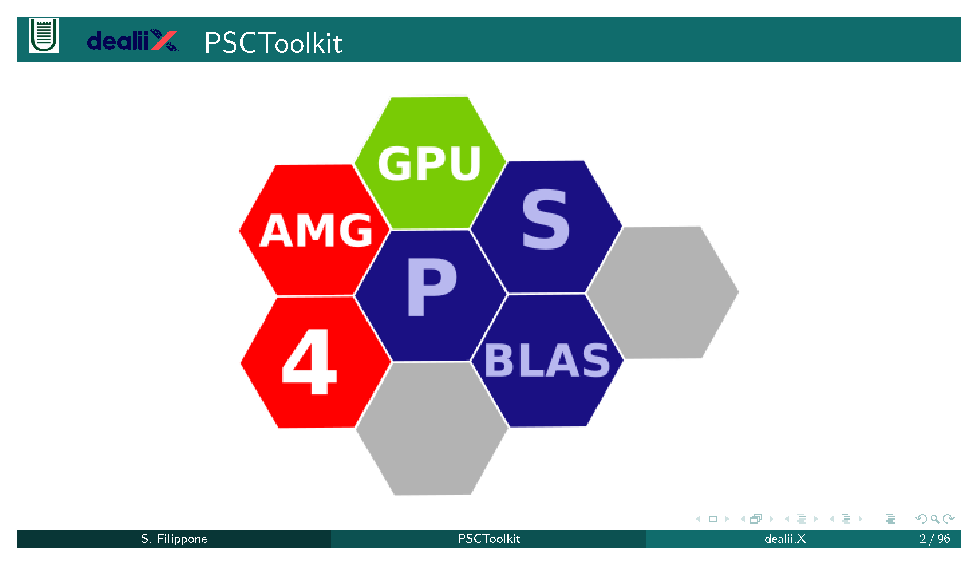
\includegraphics[width=.95\textwidth]{tutorial-002.eps}
\end{center}
\newpage
\begin{center}
  \includegraphics[width=.95\textwidth]{tutorial-003.eps}\\[2\baselineskip]
  
\includegraphics[width=.95\textwidth]{tutorial-004.eps}
\end{center}
\newpage
\begin{center}
  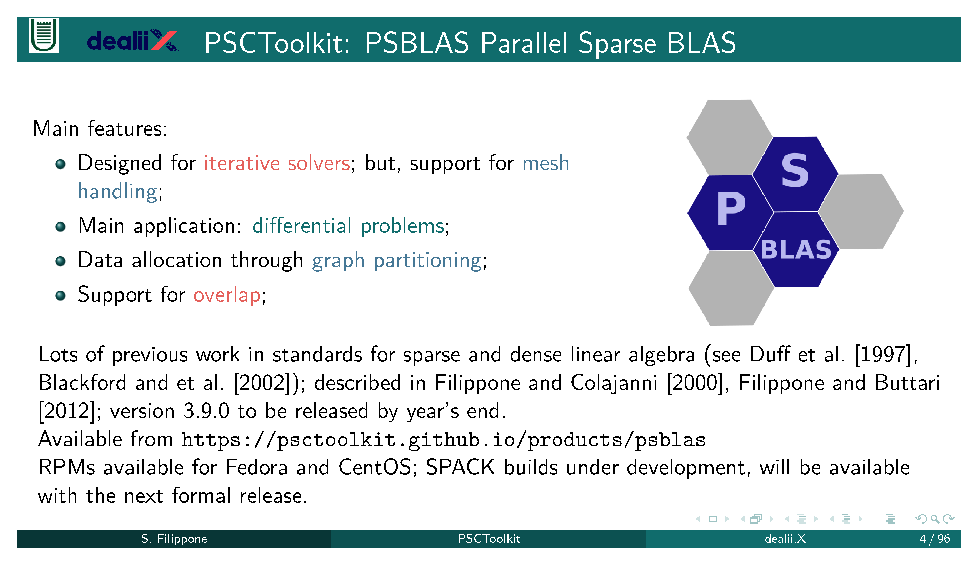
\includegraphics[width=.95\textwidth]{tutorial-005.eps}\\[2\baselineskip]
  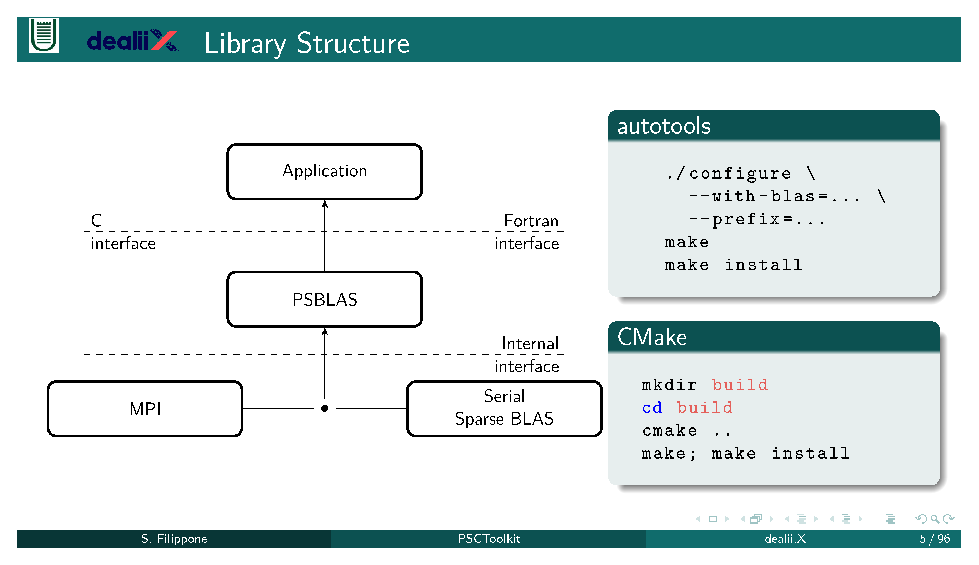
\includegraphics[width=.95\textwidth]{tutorial-006.eps}
\end{center}
\newpage
\begin{center}
  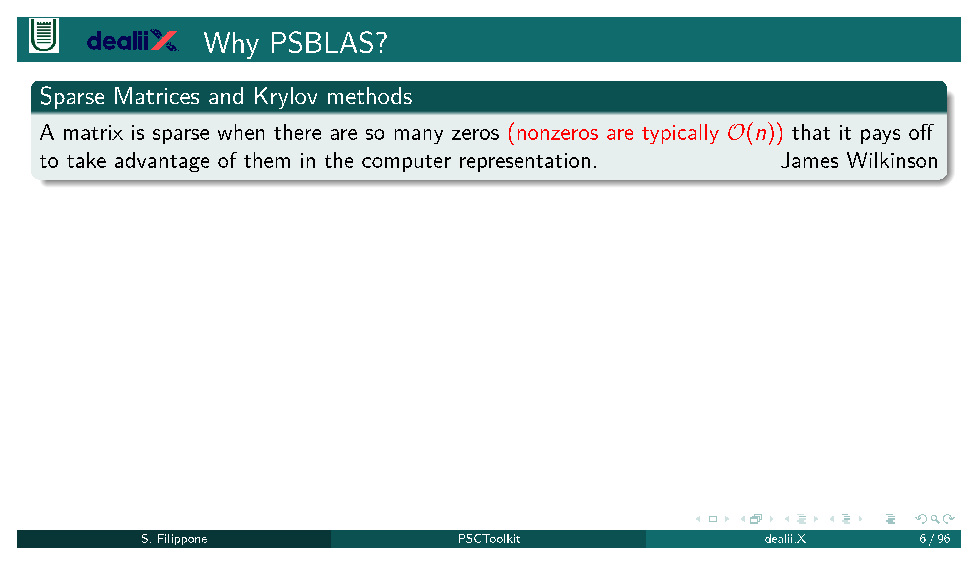
\includegraphics[width=.95\textwidth]{tutorial-007.eps}\\[2\baselineskip]
  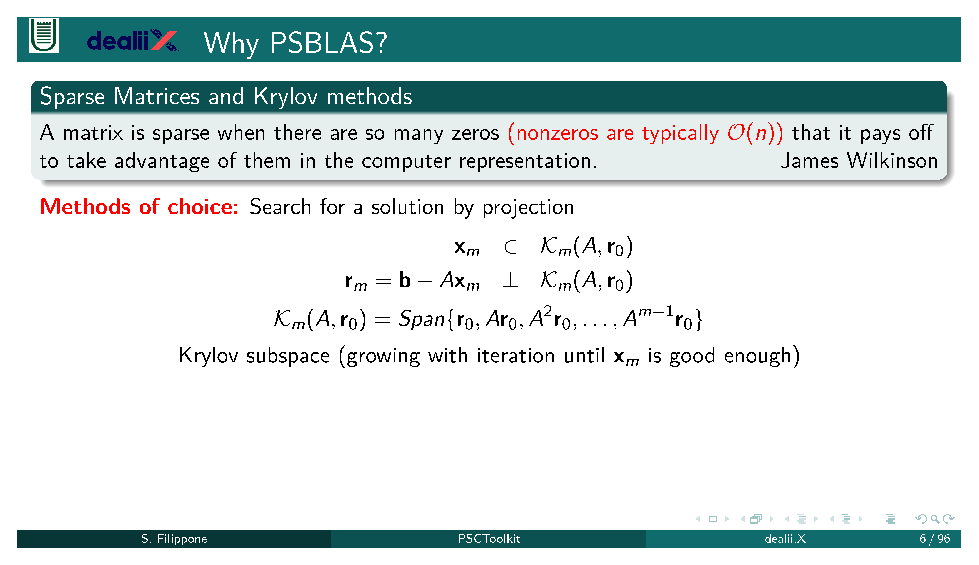
\includegraphics[width=.95\textwidth]{tutorial-008.eps}
\end{center}
\newpage
\begin{center}
  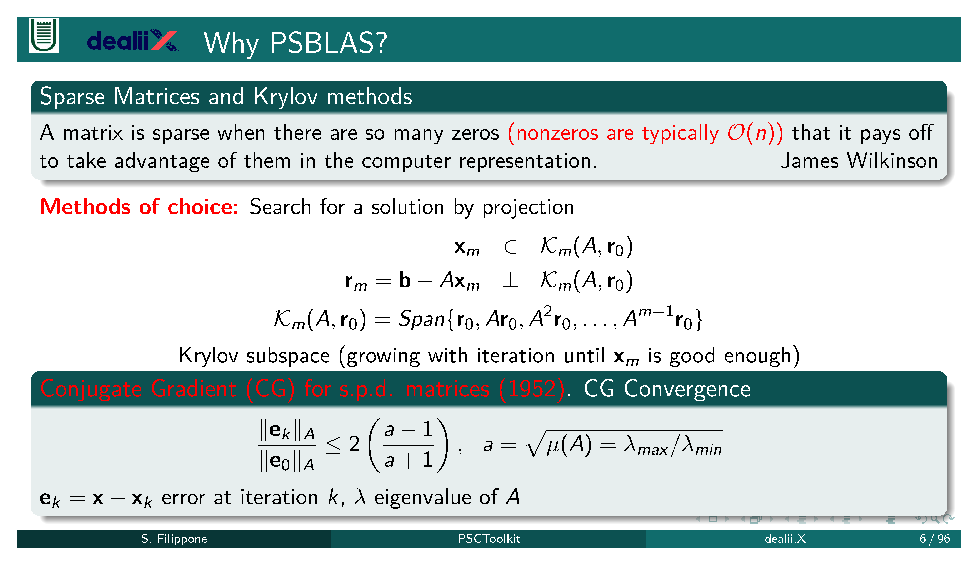
\includegraphics[width=.95\textwidth]{tutorial-009.eps}\\[2\baselineskip]
  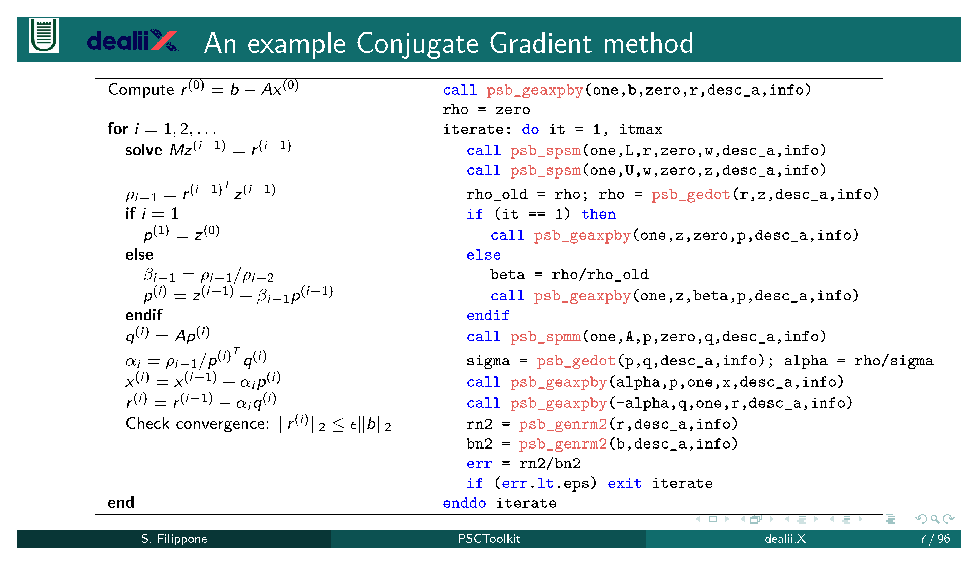
\includegraphics[width=.95\textwidth]{tutorial-010.eps}
\end{center}
\newpage
\begin{center}
  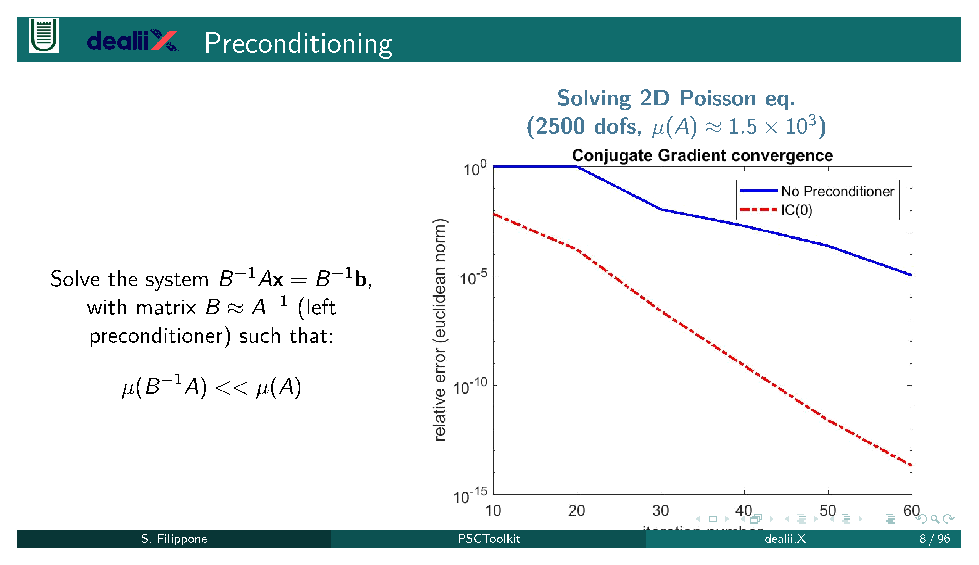
\includegraphics[width=.95\textwidth]{tutorial-011.eps}\\[2\baselineskip]
  
\includegraphics[width=.95\textwidth]{tutorial-012.eps}
\end{center}
\newpage
\begin{center}
  
\includegraphics[width=.95\textwidth]{tutorial-013.eps}\\[2\baselineskip]
  
\includegraphics[width=.95\textwidth]{tutorial-014.eps}
\end{center}
\newpage
\begin{center}
  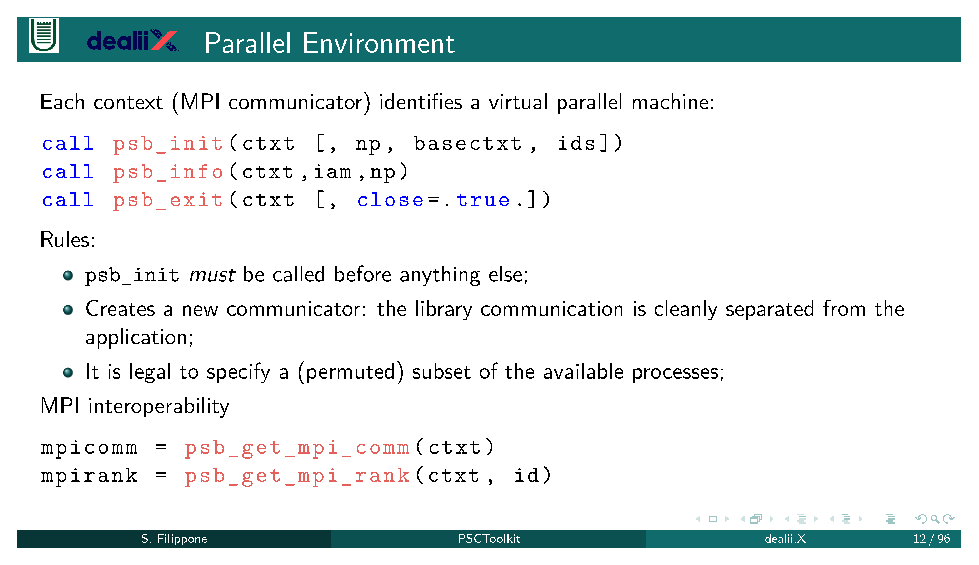
\includegraphics[width=.95\textwidth]{tutorial-015.eps}\\[2\baselineskip]
  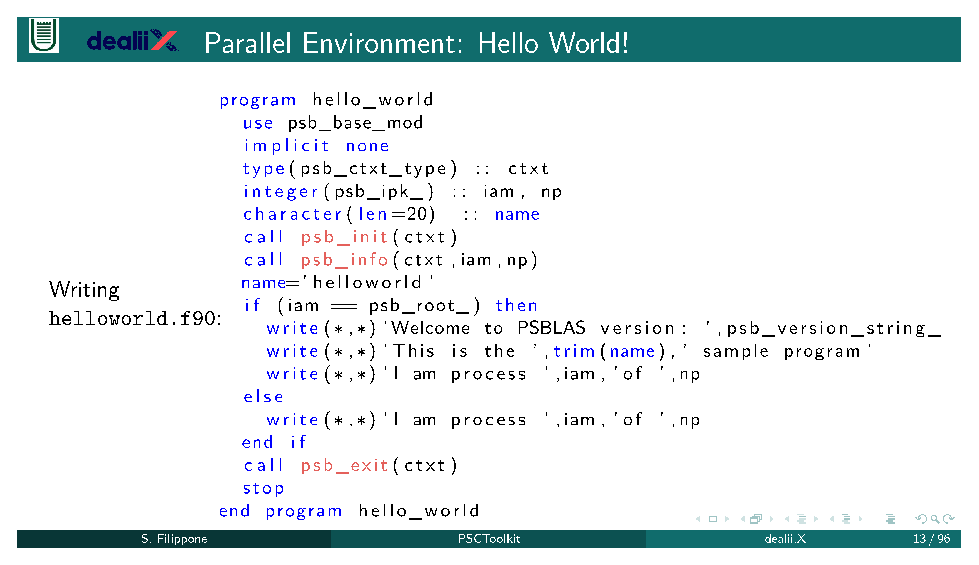
\includegraphics[width=.95\textwidth]{tutorial-016.eps}
\end{center}
\newpage
\begin{center}
  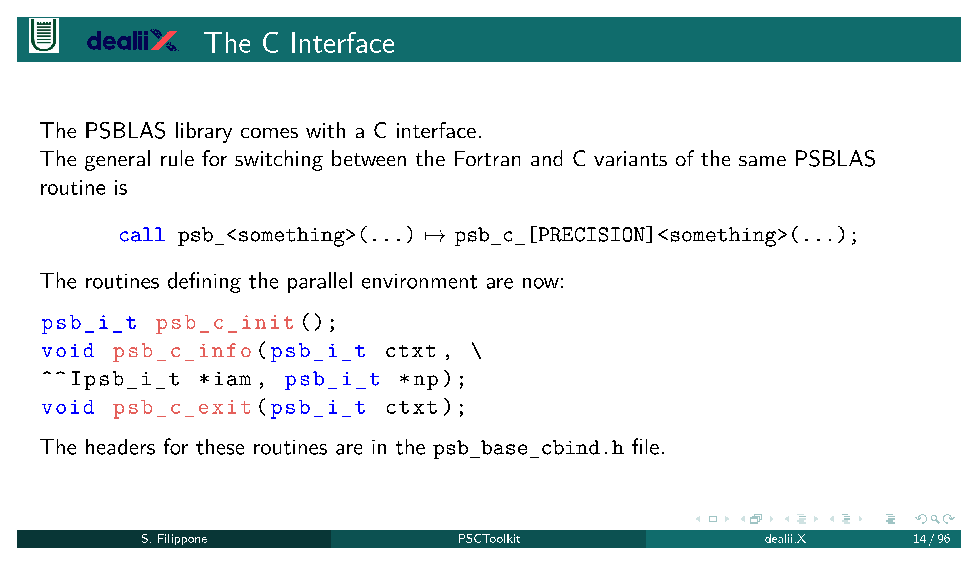
\includegraphics[width=.95\textwidth]{tutorial-017.eps}\\[2\baselineskip]
  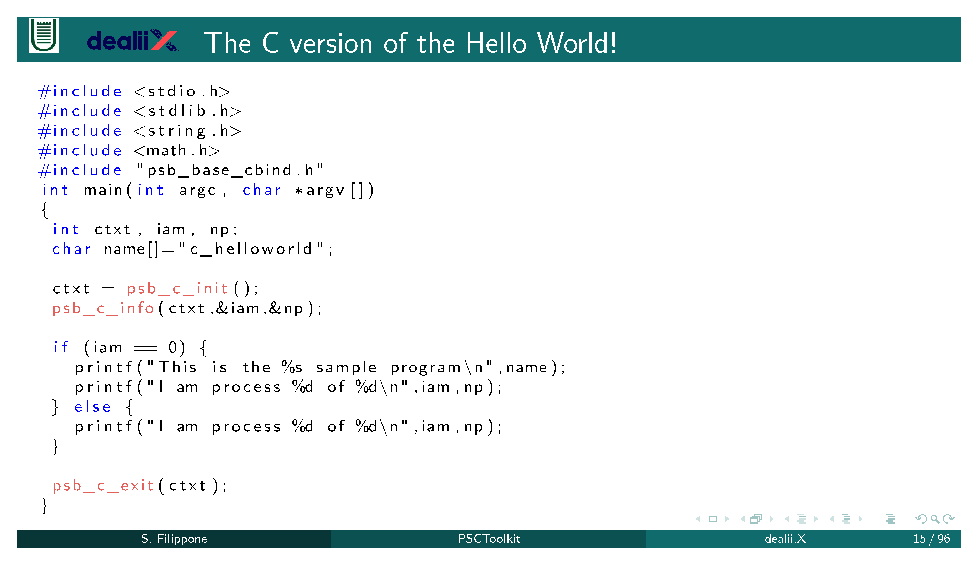
\includegraphics[width=.95\textwidth]{tutorial-018.eps}
\end{center}
\newpage
\begin{center}
  
\includegraphics[width=.95\textwidth]{tutorial-019.eps}\\[2\baselineskip]
  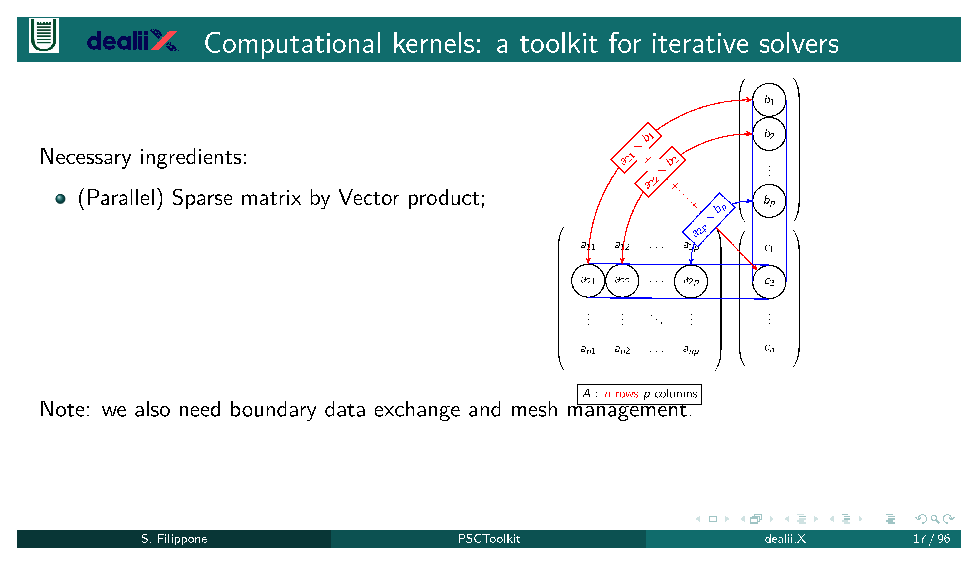
\includegraphics[width=.95\textwidth]{tutorial-020.eps}
\end{center}
\newpage
\begin{center}
  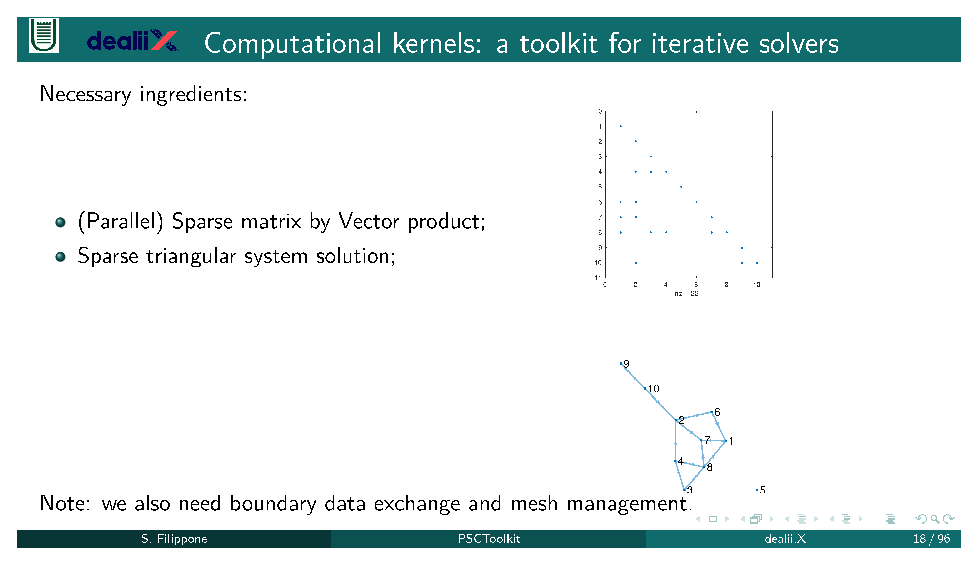
\includegraphics[width=.95\textwidth]{tutorial-021.eps}\\[2\baselineskip]
  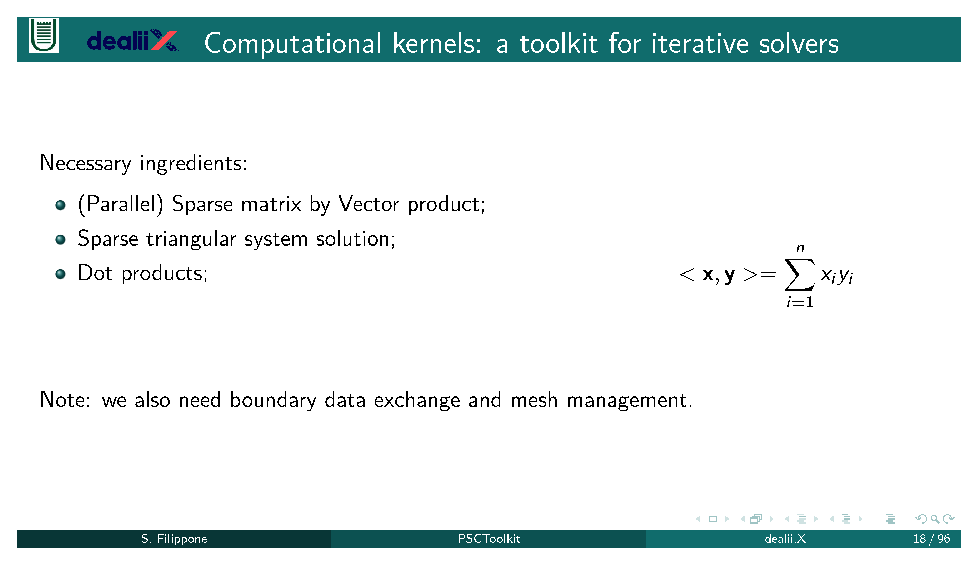
\includegraphics[width=.95\textwidth]{tutorial-022.eps}
\end{center}
\newpage
\begin{center}
  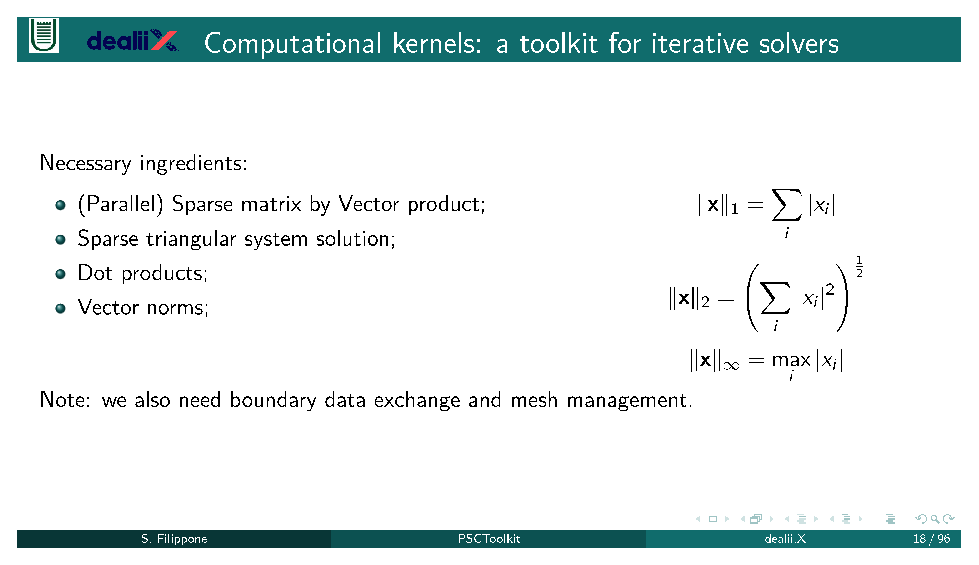
\includegraphics[width=.95\textwidth]{tutorial-023.eps}\\[2\baselineskip]
  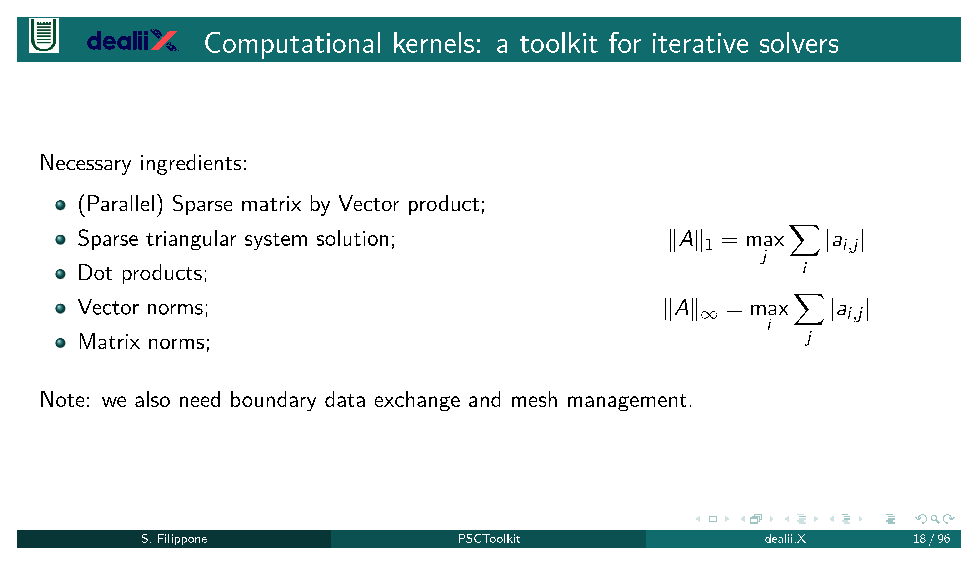
\includegraphics[width=.95\textwidth]{tutorial-024.eps}
\end{center}
\newpage
\begin{center}
  
\includegraphics[width=.95\textwidth]{tutorial-025.eps}\\[2\baselineskip]
  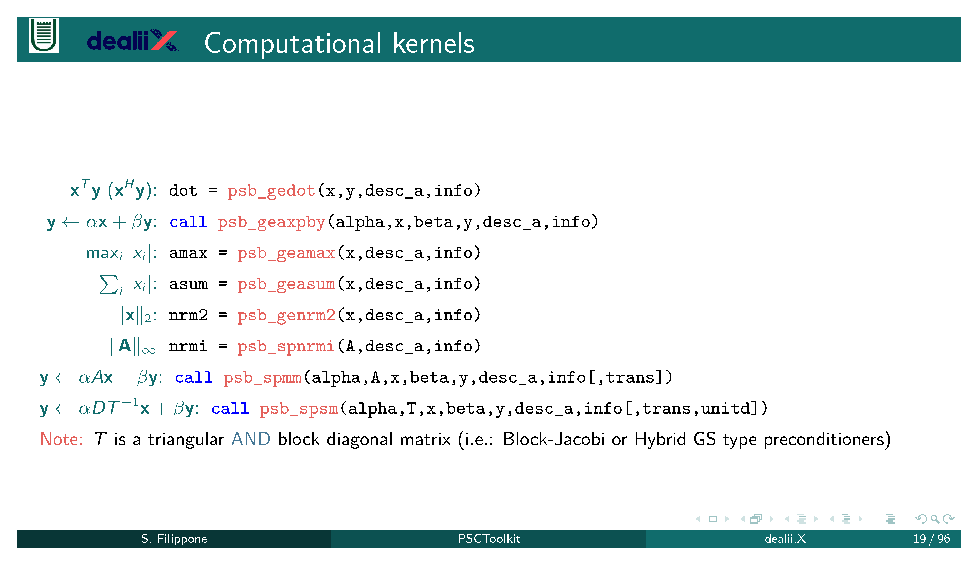
\includegraphics[width=.95\textwidth]{tutorial-026.eps}
\end{center}
\newpage
\begin{center}
  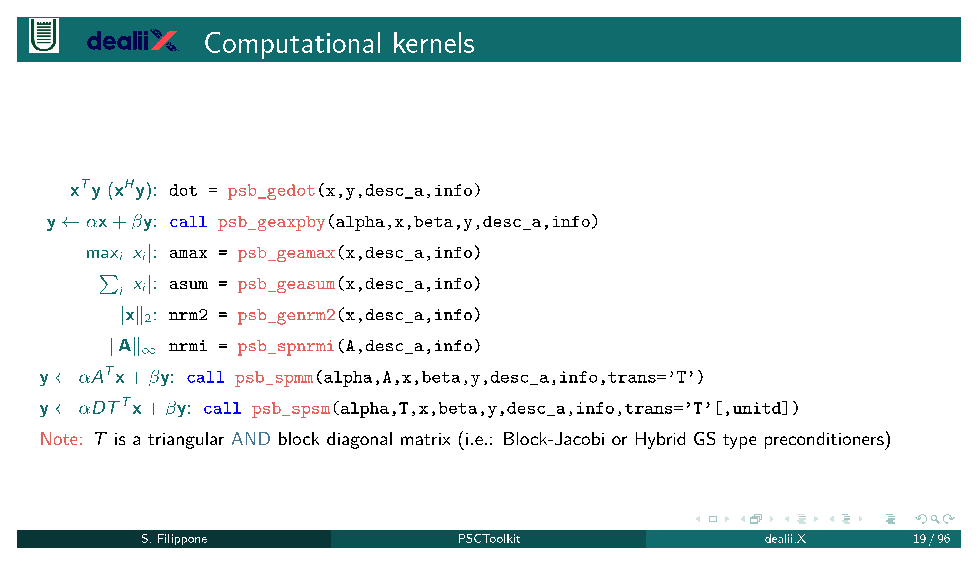
\includegraphics[width=.95\textwidth]{tutorial-027.eps}\\[2\baselineskip]
  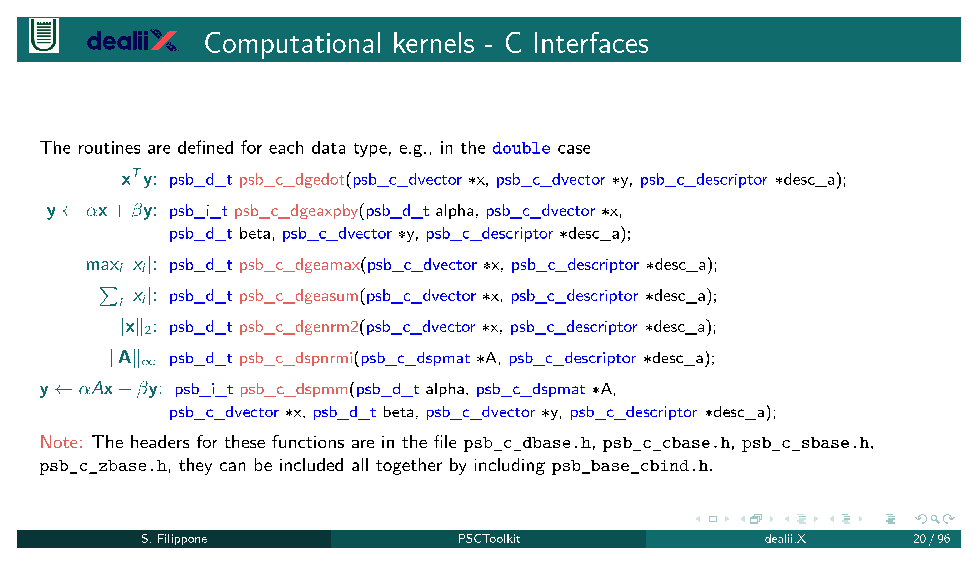
\includegraphics[width=.95\textwidth]{tutorial-028.eps}
\end{center}
\newpage
\begin{center}
  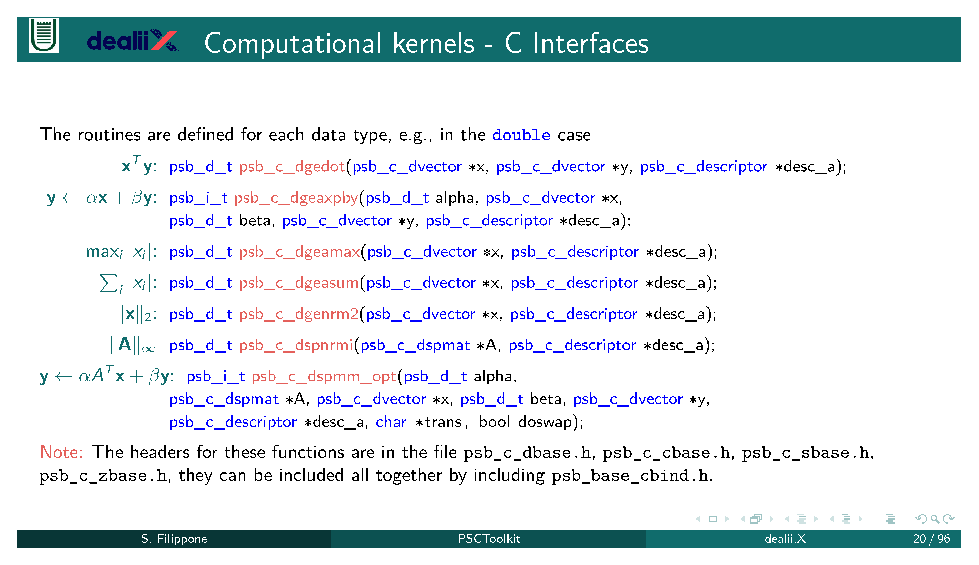
\includegraphics[width=.95\textwidth]{tutorial-029.eps}\\[2\baselineskip]
  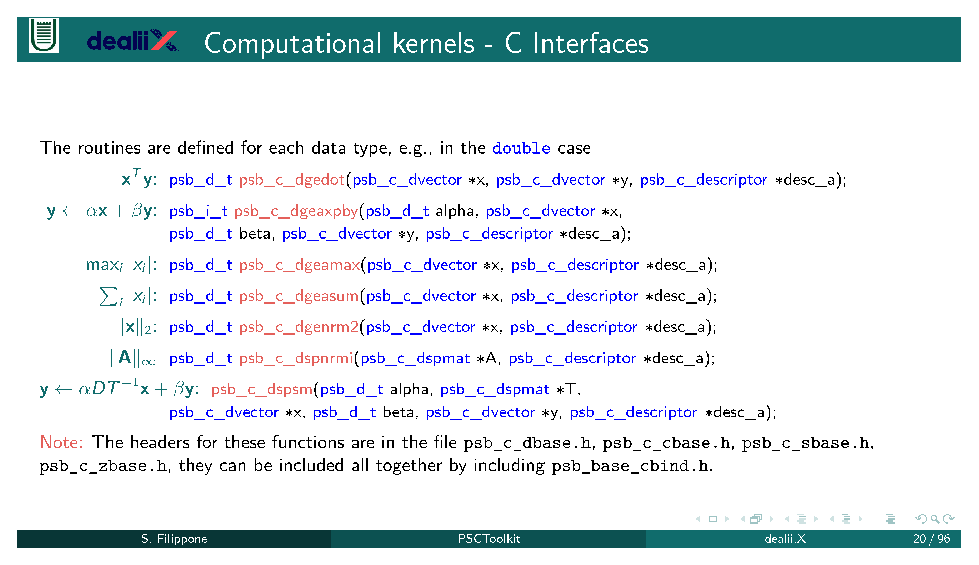
\includegraphics[width=.95\textwidth]{tutorial-030.eps}
\end{center}
\newpage
\begin{center}
  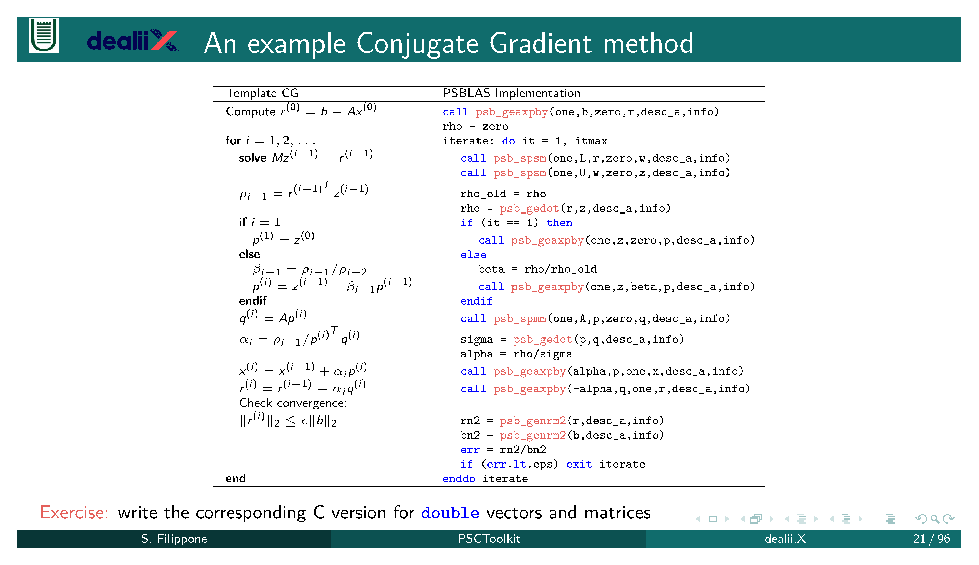
\includegraphics[width=.95\textwidth]{tutorial-031.eps}\\[2\baselineskip]
  
\includegraphics[width=.95\textwidth]{tutorial-032.eps}
\end{center}
\newpage
\begin{center}
  
\includegraphics[width=.95\textwidth]{tutorial-033.eps}\\[2\baselineskip]
  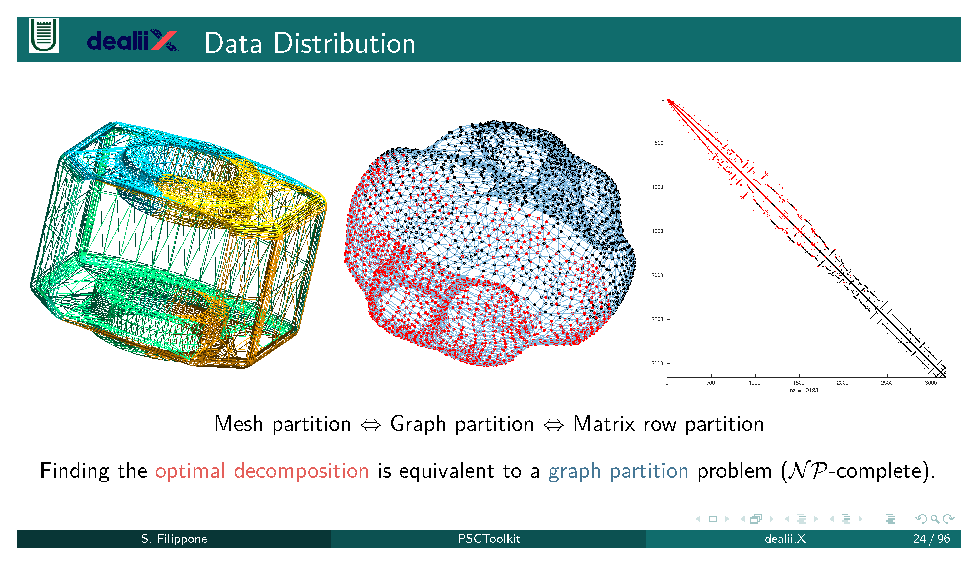
\includegraphics[width=.95\textwidth]{tutorial-034.eps}
\end{center}
\newpage
\begin{center}
  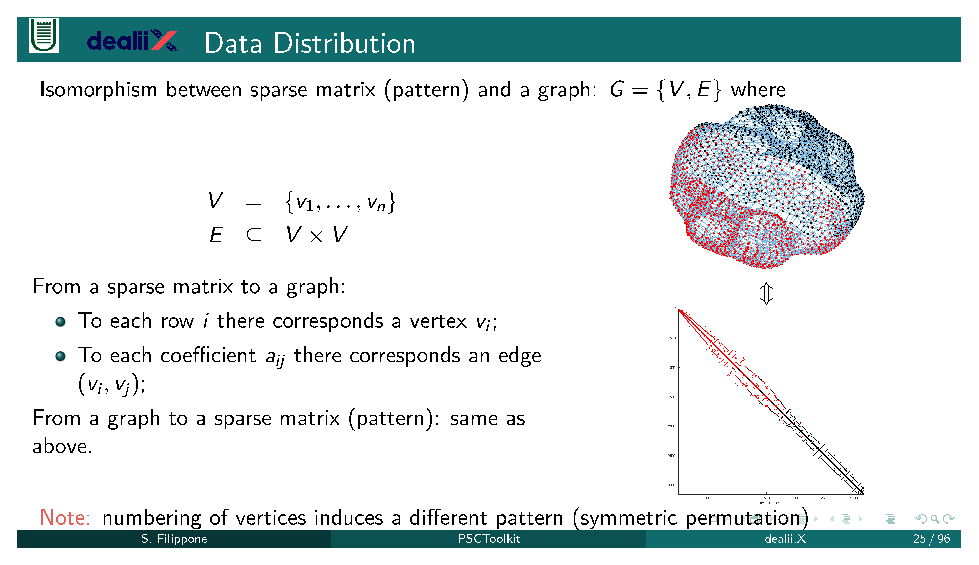
\includegraphics[width=.95\textwidth]{tutorial-035.eps}\\[2\baselineskip]
  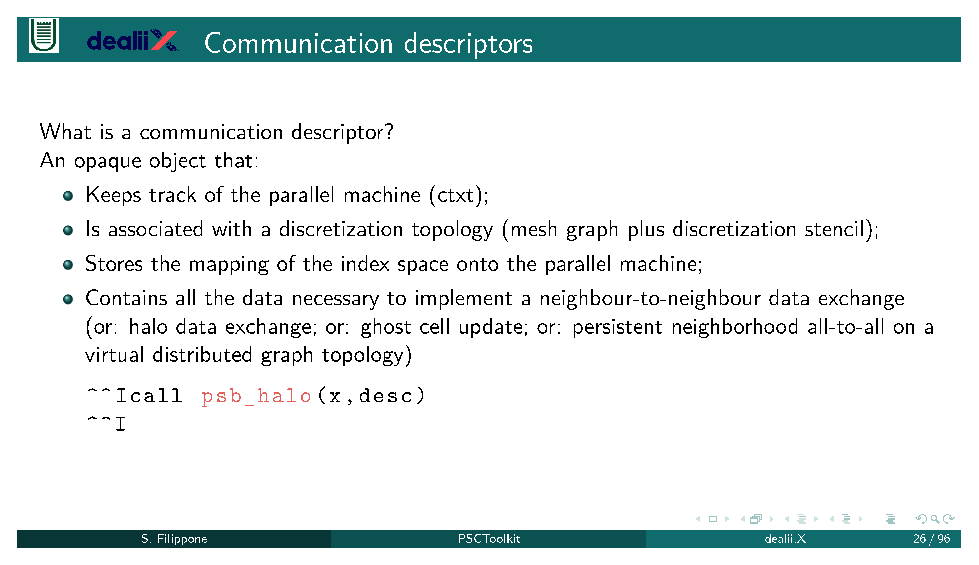
\includegraphics[width=.95\textwidth]{tutorial-036.eps}
\end{center}
\newpage
\begin{center}
  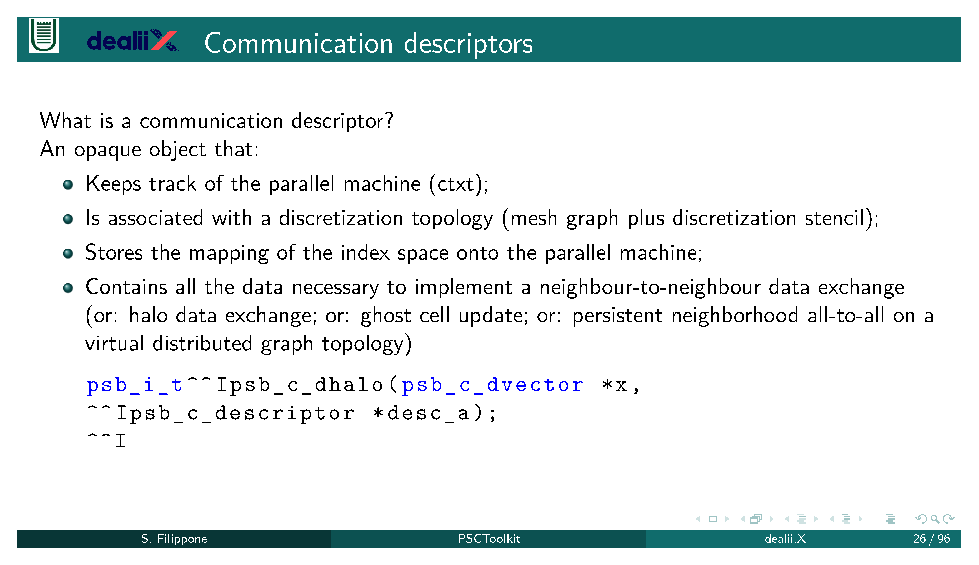
\includegraphics[width=.95\textwidth]{tutorial-037.eps}\\[2\baselineskip]
  
\includegraphics[width=.95\textwidth]{tutorial-038.eps}
\end{center}
\newpage
\begin{center}
  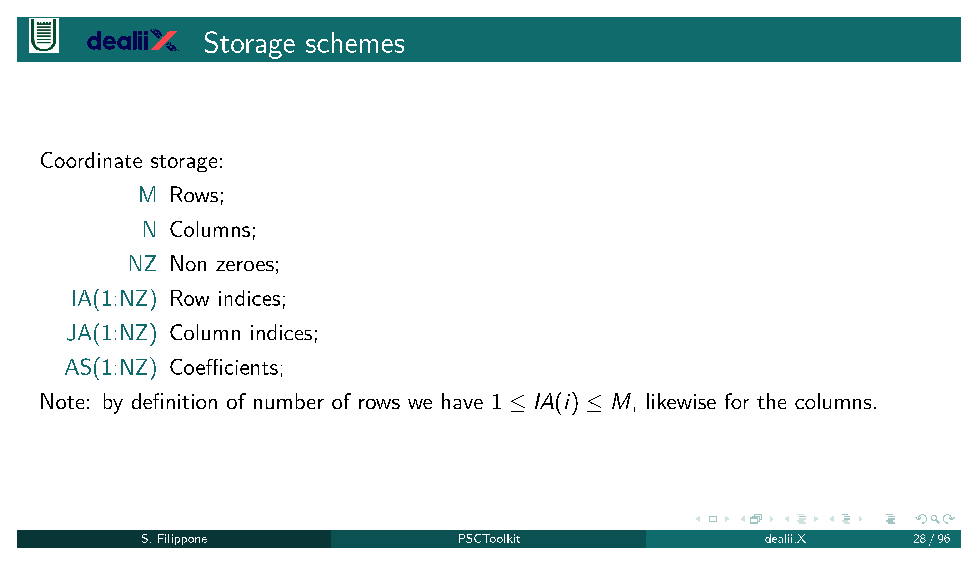
\includegraphics[width=.95\textwidth]{tutorial-039.eps}\\[2\baselineskip]
  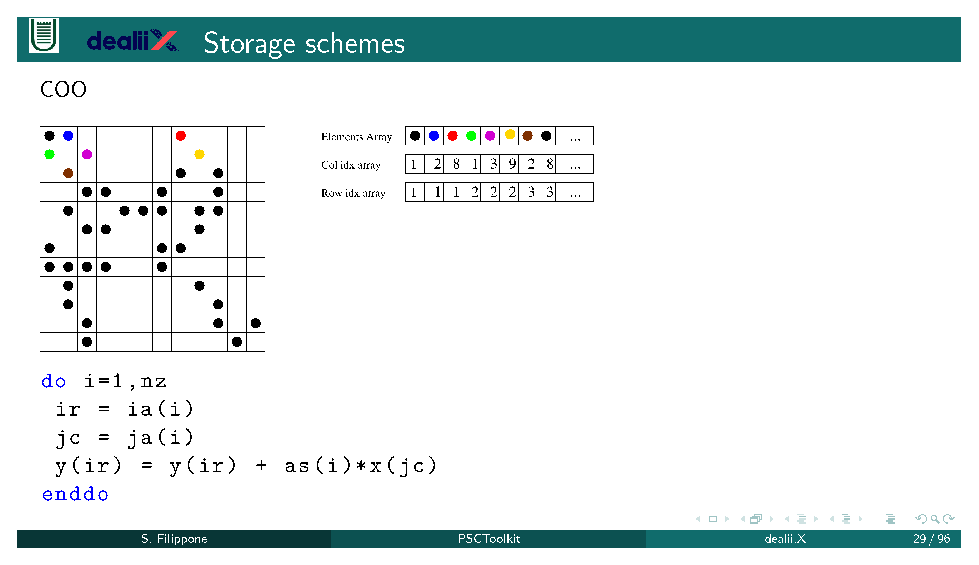
\includegraphics[width=.95\textwidth]{tutorial-040.eps}
\end{center}
\newpage
\begin{center}
  
\includegraphics[width=.95\textwidth]{tutorial-041.eps}\\[2\baselineskip]
  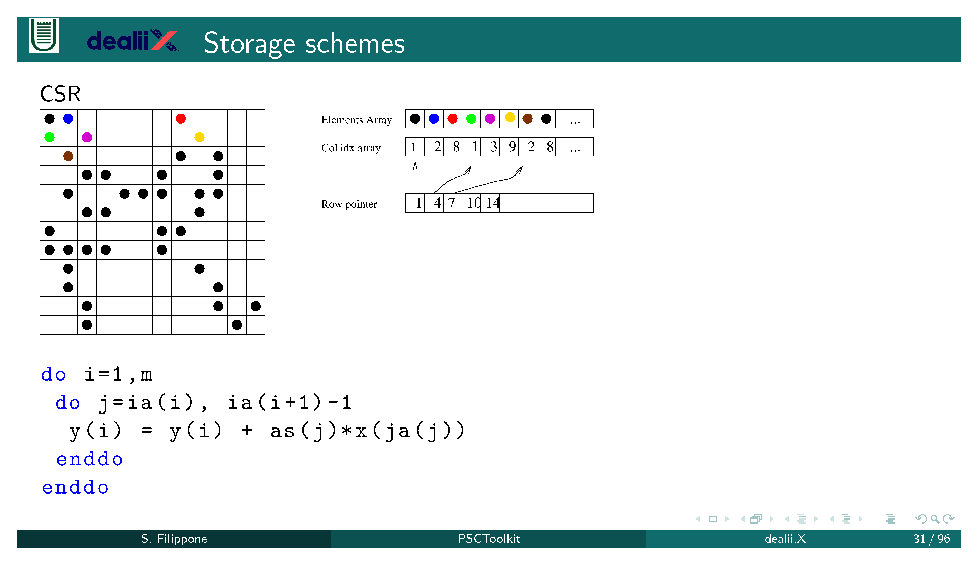
\includegraphics[width=.95\textwidth]{tutorial-042.eps}
\end{center}
\newpage
\begin{center}
  \includegraphics[width=.95\textwidth]{tutorial-043.eps}\\[2\baselineskip]
  \includegraphics[width=.95\textwidth]{tutorial-044.eps}
\end{center}
\newpage
\begin{center}
  \includegraphics[width=.95\textwidth]{tutorial-045.eps}\\[2\baselineskip]
  \includegraphics[width=.95\textwidth]{tutorial-046.eps}
\end{center}
\newpage
\begin{center}
  \includegraphics[width=.95\textwidth]{tutorial-047.eps}\\[2\baselineskip]
  \includegraphics[width=.95\textwidth]{tutorial-048.eps}
\end{center}
\newpage
\begin{center}
  \includegraphics[width=.95\textwidth]{tutorial-049.eps}\\[2\baselineskip]
  \includegraphics[width=.95\textwidth]{tutorial-050.eps}
\end{center}
\newpage
\begin{center}
  \includegraphics[width=.95\textwidth]{tutorial-051.eps}\\[2\baselineskip]
  \includegraphics[width=.95\textwidth]{tutorial-052.eps}
\end{center}
\newpage
\begin{center}
  \includegraphics[width=.95\textwidth]{tutorial-053.eps}\\[2\baselineskip]
  \includegraphics[width=.95\textwidth]{tutorial-054.eps}
\end{center}
\newpage
\begin{center}
  \includegraphics[width=.95\textwidth]{tutorial-055.eps}\\[2\baselineskip]
  \includegraphics[width=.95\textwidth]{tutorial-056.eps}
\end{center}
\newpage
\begin{center}
  \includegraphics[width=.95\textwidth]{tutorial-057.eps}\\[2\baselineskip]
  \includegraphics[width=.95\textwidth]{tutorial-058.eps}
\end{center}
\newpage
\begin{center}
  \includegraphics[width=.95\textwidth]{tutorial-059.eps}\\[2\baselineskip]
  \includegraphics[width=.95\textwidth]{tutorial-060.eps}
\end{center}
\newpage
\begin{center}
  \includegraphics[width=.95\textwidth]{tutorial-061.eps}\\[2\baselineskip]
  \includegraphics[width=.95\textwidth]{tutorial-062.eps}
\end{center}
\newpage
\begin{center}
  \includegraphics[width=.95\textwidth]{tutorial-063.eps}\\[2\baselineskip]
  \includegraphics[width=.95\textwidth]{tutorial-064.eps}
\end{center}
\newpage
\begin{center}
  \includegraphics[width=.95\textwidth]{tutorial-065.eps}\\[2\baselineskip]
  \includegraphics[width=.95\textwidth]{tutorial-066.eps}
\end{center}
\newpage
\begin{center}
  \includegraphics[width=.95\textwidth]{tutorial-067.eps}\\[2\baselineskip]
  \includegraphics[width=.95\textwidth]{tutorial-068.eps}
\end{center}
\newpage
\begin{center}
  \includegraphics[width=.95\textwidth]{tutorial-069.eps}\\[2\baselineskip]
  \includegraphics[width=.95\textwidth]{tutorial-070.eps}
\end{center}
\newpage
\begin{center}
  \includegraphics[width=.95\textwidth]{tutorial-071.eps}\\[2\baselineskip]
  \includegraphics[width=.95\textwidth]{tutorial-072.eps}
\end{center}
\newpage
\begin{center}
  \includegraphics[width=.95\textwidth]{tutorial-073.eps}\\[2\baselineskip]
  \includegraphics[width=.95\textwidth]{tutorial-074.eps}
\end{center}
\newpage
\begin{center}
  \includegraphics[width=.95\textwidth]{tutorial-075.eps}\\[2\baselineskip]
  \includegraphics[width=.95\textwidth]{tutorial-076.eps}
\end{center}
\newpage
\begin{center}
  \includegraphics[width=.95\textwidth]{tutorial-077.eps}\\[2\baselineskip]
  \includegraphics[width=.95\textwidth]{tutorial-078.eps}
\end{center}
\newpage
\begin{center}
  \includegraphics[width=.95\textwidth]{tutorial-079.eps}\\[2\baselineskip]
  \includegraphics[width=.95\textwidth]{tutorial-080.eps}
\end{center}
\newpage
\begin{center}
  \includegraphics[width=.95\textwidth]{tutorial-081.eps}\\[2\baselineskip]
  \includegraphics[width=.95\textwidth]{tutorial-082.eps}
\end{center}
\newpage
\begin{center}
  \includegraphics[width=.95\textwidth]{tutorial-083.eps}\\[2\baselineskip]
  \includegraphics[width=.95\textwidth]{tutorial-084.eps}
\end{center}
\newpage
\begin{center}
  \includegraphics[width=.95\textwidth]{tutorial-085.eps}\\[2\baselineskip]
  \includegraphics[width=.95\textwidth]{tutorial-086.eps}
\end{center}
\newpage
\begin{center}
  \includegraphics[width=.95\textwidth]{tutorial-087.eps}\\[2\baselineskip]
  \includegraphics[width=.95\textwidth]{tutorial-088.eps}
\end{center}
\newpage
\begin{center}
  \includegraphics[width=.95\textwidth]{tutorial-089.eps}\\[2\baselineskip]
  \includegraphics[width=.95\textwidth]{tutorial-090.eps}
\end{center}
\newpage
\begin{center}
  \includegraphics[width=.95\textwidth]{tutorial-091.eps}\\[2\baselineskip]
  \includegraphics[width=.95\textwidth]{tutorial-092.eps}
\end{center}
\newpage
\begin{center}
  \includegraphics[width=.95\textwidth]{tutorial-093.eps}\\[2\baselineskip]
  \includegraphics[width=.95\textwidth]{tutorial-094.eps}
\end{center}
\newpage
\begin{center}
  \includegraphics[width=.95\textwidth]{tutorial-095.eps}\\[2\baselineskip]
  \includegraphics[width=.95\textwidth]{tutorial-096.eps}
\end{center}
\newpage
\begin{center}
  \includegraphics[width=.95\textwidth]{tutorial-097.eps}\\[2\baselineskip]
  \includegraphics[width=.95\textwidth]{tutorial-098.eps}
\end{center}
\newpage
\begin{center}
  \includegraphics[width=.95\textwidth]{tutorial-099.eps}\\[2\baselineskip]
  \includegraphics[width=.95\textwidth]{tutorial-100.eps}
\end{center}
\newpage
\begin{center}
  \includegraphics[width=.95\textwidth]{tutorial-101.eps}\\[2\baselineskip]
  \includegraphics[width=.95\textwidth]{tutorial-102.eps}
\end{center}
\newpage
\begin{center}
  \includegraphics[width=.95\textwidth]{tutorial-103.eps}\\[2\baselineskip]
  \includegraphics[width=.95\textwidth]{tutorial-104.eps}
\end{center}
\newpage
\begin{center}
  \includegraphics[width=.95\textwidth]{tutorial-105.eps}\\[2\baselineskip]
  \includegraphics[width=.95\textwidth]{tutorial-106.eps}
\end{center}
\newpage
\begin{center}
  \includegraphics[width=.95\textwidth]{tutorial-107.eps}\\[2\baselineskip]
  \includegraphics[width=.95\textwidth]{tutorial-108.eps}
\end{center}
\newpage
\begin{center}
  \includegraphics[width=.95\textwidth]{tutorial-109.eps}\\[2\baselineskip]
  \includegraphics[width=.95\textwidth]{tutorial-110.eps}
\end{center}
\newpage
\begin{center}
  \includegraphics[width=.95\textwidth]{tutorial-111.eps}\\[2\baselineskip]
  \includegraphics[width=.95\textwidth]{tutorial-112.eps}
\end{center}
\newpage
\begin{center}
  \includegraphics[width=.95\textwidth]{tutorial-113.eps}\\[2\baselineskip]
  \includegraphics[width=.95\textwidth]{tutorial-114.eps}
\end{center}
\newpage
\begin{center}
  \includegraphics[width=.95\textwidth]{tutorial-115.eps}\\[2\baselineskip]
  \includegraphics[width=.95\textwidth]{tutorial-116.eps}
\end{center}
\newpage
\begin{center}
  \includegraphics[width=.95\textwidth]{tutorial-117.eps}\\[2\baselineskip]
  \includegraphics[width=.95\textwidth]{tutorial-118.eps}
\end{center}
\newpage
\begin{center}
  \includegraphics[width=.95\textwidth]{tutorial-119.eps}\\[2\baselineskip]
  \includegraphics[width=.95\textwidth]{tutorial-120.eps}
\end{center}
\newpage
\begin{center}
  \includegraphics[width=.95\textwidth]{tutorial-121.eps}\\[2\baselineskip]
  \includegraphics[width=.95\textwidth]{tutorial-122.eps}
\end{center}
\newpage
\begin{center}
  \includegraphics[width=.95\textwidth]{tutorial-123.eps}\\[2\baselineskip]
  \includegraphics[width=.95\textwidth]{tutorial-124.eps}
\end{center}
\newpage
\begin{center}
  \includegraphics[width=.95\textwidth]{tutorial-125.eps}\\[2\baselineskip]
  \includegraphics[width=.95\textwidth]{tutorial-126.eps}
\end{center}



\label{MyLastPage}

\end{document}
